% Options for packages loaded elsewhere
\PassOptionsToPackage{unicode}{hyperref}
\PassOptionsToPackage{hyphens}{url}
%
\documentclass[
]{article}
\usepackage{lmodern}
\usepackage{amssymb,amsmath}
\usepackage{ifxetex,ifluatex}
\ifnum 0\ifxetex 1\fi\ifluatex 1\fi=0 % if pdftex
  \usepackage[T1]{fontenc}
  \usepackage[utf8]{inputenc}
  \usepackage{textcomp} % provide euro and other symbols
\else % if luatex or xetex
  \usepackage{unicode-math}
  \defaultfontfeatures{Scale=MatchLowercase}
  \defaultfontfeatures[\rmfamily]{Ligatures=TeX,Scale=1}
\fi
% Use upquote if available, for straight quotes in verbatim environments
\IfFileExists{upquote.sty}{\usepackage{upquote}}{}
\IfFileExists{microtype.sty}{% use microtype if available
  \usepackage[]{microtype}
  \UseMicrotypeSet[protrusion]{basicmath} % disable protrusion for tt fonts
}{}
\makeatletter
\@ifundefined{KOMAClassName}{% if non-KOMA class
  \IfFileExists{parskip.sty}{%
    \usepackage{parskip}
  }{% else
    \setlength{\parindent}{0pt}
    \setlength{\parskip}{6pt plus 2pt minus 1pt}}
}{% if KOMA class
  \KOMAoptions{parskip=half}}
\makeatother
\usepackage{xcolor}
\IfFileExists{xurl.sty}{\usepackage{xurl}}{} % add URL line breaks if available
\IfFileExists{bookmark.sty}{\usepackage{bookmark}}{\usepackage{hyperref}}
\hypersetup{
  pdftitle={file\_pdf},
  pdfauthor={Daniel Pagotto},
  hidelinks,
  pdfcreator={LaTeX via pandoc}}
\urlstyle{same} % disable monospaced font for URLs
\usepackage[margin=1in]{geometry}
\usepackage{color}
\usepackage{fancyvrb}
\newcommand{\VerbBar}{|}
\newcommand{\VERB}{\Verb[commandchars=\\\{\}]}
\DefineVerbatimEnvironment{Highlighting}{Verbatim}{commandchars=\\\{\}}
% Add ',fontsize=\small' for more characters per line
\usepackage{framed}
\definecolor{shadecolor}{RGB}{248,248,248}
\newenvironment{Shaded}{\begin{snugshade}}{\end{snugshade}}
\newcommand{\AlertTok}[1]{\textcolor[rgb]{0.94,0.16,0.16}{#1}}
\newcommand{\AnnotationTok}[1]{\textcolor[rgb]{0.56,0.35,0.01}{\textbf{\textit{#1}}}}
\newcommand{\AttributeTok}[1]{\textcolor[rgb]{0.77,0.63,0.00}{#1}}
\newcommand{\BaseNTok}[1]{\textcolor[rgb]{0.00,0.00,0.81}{#1}}
\newcommand{\BuiltInTok}[1]{#1}
\newcommand{\CharTok}[1]{\textcolor[rgb]{0.31,0.60,0.02}{#1}}
\newcommand{\CommentTok}[1]{\textcolor[rgb]{0.56,0.35,0.01}{\textit{#1}}}
\newcommand{\CommentVarTok}[1]{\textcolor[rgb]{0.56,0.35,0.01}{\textbf{\textit{#1}}}}
\newcommand{\ConstantTok}[1]{\textcolor[rgb]{0.00,0.00,0.00}{#1}}
\newcommand{\ControlFlowTok}[1]{\textcolor[rgb]{0.13,0.29,0.53}{\textbf{#1}}}
\newcommand{\DataTypeTok}[1]{\textcolor[rgb]{0.13,0.29,0.53}{#1}}
\newcommand{\DecValTok}[1]{\textcolor[rgb]{0.00,0.00,0.81}{#1}}
\newcommand{\DocumentationTok}[1]{\textcolor[rgb]{0.56,0.35,0.01}{\textbf{\textit{#1}}}}
\newcommand{\ErrorTok}[1]{\textcolor[rgb]{0.64,0.00,0.00}{\textbf{#1}}}
\newcommand{\ExtensionTok}[1]{#1}
\newcommand{\FloatTok}[1]{\textcolor[rgb]{0.00,0.00,0.81}{#1}}
\newcommand{\FunctionTok}[1]{\textcolor[rgb]{0.00,0.00,0.00}{#1}}
\newcommand{\ImportTok}[1]{#1}
\newcommand{\InformationTok}[1]{\textcolor[rgb]{0.56,0.35,0.01}{\textbf{\textit{#1}}}}
\newcommand{\KeywordTok}[1]{\textcolor[rgb]{0.13,0.29,0.53}{\textbf{#1}}}
\newcommand{\NormalTok}[1]{#1}
\newcommand{\OperatorTok}[1]{\textcolor[rgb]{0.81,0.36,0.00}{\textbf{#1}}}
\newcommand{\OtherTok}[1]{\textcolor[rgb]{0.56,0.35,0.01}{#1}}
\newcommand{\PreprocessorTok}[1]{\textcolor[rgb]{0.56,0.35,0.01}{\textit{#1}}}
\newcommand{\RegionMarkerTok}[1]{#1}
\newcommand{\SpecialCharTok}[1]{\textcolor[rgb]{0.00,0.00,0.00}{#1}}
\newcommand{\SpecialStringTok}[1]{\textcolor[rgb]{0.31,0.60,0.02}{#1}}
\newcommand{\StringTok}[1]{\textcolor[rgb]{0.31,0.60,0.02}{#1}}
\newcommand{\VariableTok}[1]{\textcolor[rgb]{0.00,0.00,0.00}{#1}}
\newcommand{\VerbatimStringTok}[1]{\textcolor[rgb]{0.31,0.60,0.02}{#1}}
\newcommand{\WarningTok}[1]{\textcolor[rgb]{0.56,0.35,0.01}{\textbf{\textit{#1}}}}
\usepackage{longtable,booktabs}
% Correct order of tables after \paragraph or \subparagraph
\usepackage{etoolbox}
\makeatletter
\patchcmd\longtable{\par}{\if@noskipsec\mbox{}\fi\par}{}{}
\makeatother
% Allow footnotes in longtable head/foot
\IfFileExists{footnotehyper.sty}{\usepackage{footnotehyper}}{\usepackage{footnote}}
\makesavenoteenv{longtable}
\usepackage{graphicx,grffile}
\makeatletter
\def\maxwidth{\ifdim\Gin@nat@width>\linewidth\linewidth\else\Gin@nat@width\fi}
\def\maxheight{\ifdim\Gin@nat@height>\textheight\textheight\else\Gin@nat@height\fi}
\makeatother
% Scale images if necessary, so that they will not overflow the page
% margins by default, and it is still possible to overwrite the defaults
% using explicit options in \includegraphics[width, height, ...]{}
\setkeys{Gin}{width=\maxwidth,height=\maxheight,keepaspectratio}
% Set default figure placement to htbp
\makeatletter
\def\fps@figure{htbp}
\makeatother
\setlength{\emergencystretch}{3em} % prevent overfull lines
\providecommand{\tightlist}{%
  \setlength{\itemsep}{0pt}\setlength{\parskip}{0pt}}
\setcounter{secnumdepth}{-\maxdimen} % remove section numbering

\title{file\_pdf}
\author{Daniel Pagotto}
\date{21/06/2021}

\begin{document}
\maketitle

\hypertarget{agradecimentos}{%
\section{Agradecimentos}\label{agradecimentos}}

\begin{figure}

{\centering 
\includegraphics[width=1\linewidth,height=1\textheight]{imagem/agradecimentos} 

}

\caption{ }\label{fig:agradecimentos, figures-side}
\end{figure}

\hypertarget{about-me}{%
\section{About me!}\label{about-me}}

\begin{itemize}
\tightlist
\item
  Bacharel em Administração (UnB), Mestre em Administração (UFG),
  doutorando em Administração (UnB)
\item
  Já desenvolveu projetos em áreas, como: empreendedorismo,
  gestão/políticas públicas, inovação na saúde
\item
  Há aproximadamente dois anos tem utilizado R rotineiramente em suas
  atividades de trabalho e ministrado cursos para a comunidade de R
\end{itemize}

\begin{figure}

{\centering 
\includegraphics[width=0.75\linewidth,height=0.65\textheight]{imagem/logos-lape-cigets} 

}

\caption{ }\label{fig:gatas, figures-side}
\end{figure}

\hypertarget{divisuxe3o-do-curso}{%
\section{Divisão do curso}\label{divisuxe3o-do-curso}}

\begin{itemize}
\tightlist
\item
  \textbf{Módulo 1: conceitos básicos de R}

  \begin{itemize}
  \tightlist
  \item
    Cálculos básicos
  \end{itemize}
\item
  Tipos de variáveis e objetos
\item
  O pacote dplyr para manipulação de dataframes
\item
  O pacote ggplot2 para visualização de dados
\item
  \textbf{Módulo 2: usando o R para explorar o Global Entrepreneurship
  Monitor (GEM)}

  \begin{itemize}
  \tightlist
  \item
    Compreendedo as bases
  \end{itemize}
\item
  Tratando as bases
\item
  Análise Exploratória dos Dados do GEM
\item
  \textbf{Módulo 3: usando o R para explorar o Panel Study of
  Entrepreneurial Dynamics (PSED)}

  \begin{itemize}
  \tightlist
  \item
    Compreendendo a base
  \end{itemize}
\item
  Tratando a base
\item
  Análise Exploratória dos Dados do PSED
\end{itemize}

\hypertarget{objetivos-do-muxf3dulo-1}{%
\section{Objetivos do módulo 1}\label{objetivos-do-muxf3dulo-1}}

\begin{itemize}
\tightlist
\item
  Demonstrar a relevância do uso do R
\item
  Aplicar operações básicas
\item
  Descrever tipos de objetos
\item
  Descrever tipos de variáveis
\item
  Aplicar funções para manipular dataframes
\item
  Aplicar funções para visualização de dados
\end{itemize}

\hypertarget{por-que-usar-o-r}{%
\section{Por que usar o R?}\label{por-que-usar-o-r}}

\begin{center}\includegraphics[width=0.8\linewidth,height=0.8\textheight]{https://media.giphy.com/media/WMODmi5AX9ZEQ/giphy} \end{center}

\hypertarget{o-r-me-duxe1-medo}{%
\section{O R me dá medo}\label{o-r-me-duxe1-medo}}

Nunca programei\ldots{} vou conseguir?

\begin{figure}

{\centering 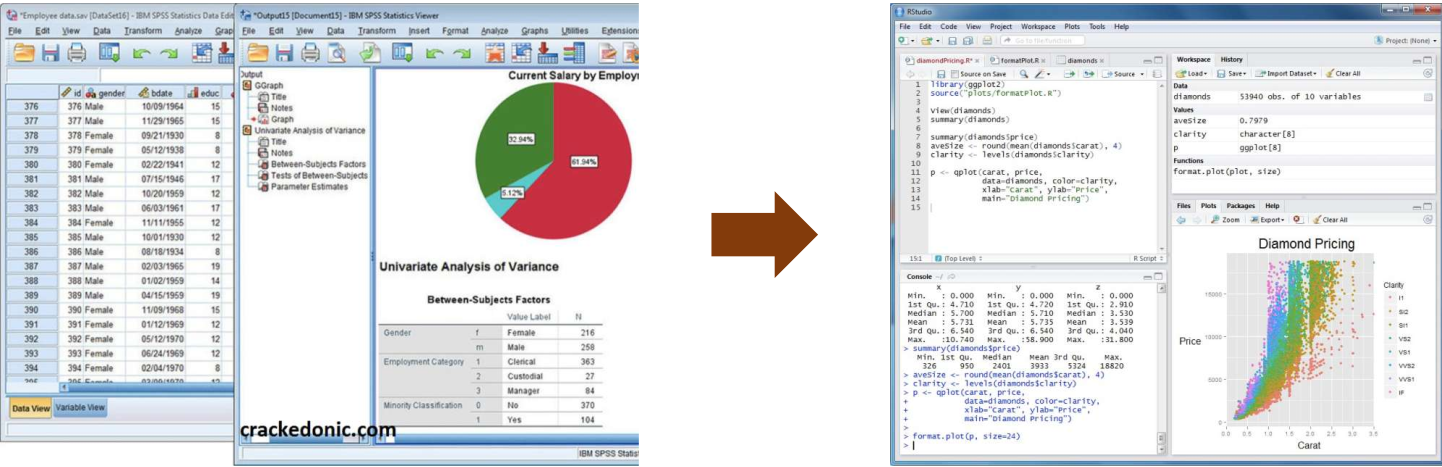
\includegraphics[width=1\linewidth,height=1\textheight]{imagem/r_spss} 

}

\caption{ }\label{fig:r_spss, figures-side}
\end{figure}

``Não consigo entender esse bando de código\ldots{}''

``É tão mais fácil usar o SPSS que basta alguns cliques e me gera
resultados rapidamente\ldots{}''

``Toda vez que tento usar R é erro para cá, erro para lá\ldots{}''

\hypertarget{r-e-ciuxeancia-de-dados}{%
\section{R e ciência de dados}\label{r-e-ciuxeancia-de-dados}}

\begin{figure}

{\centering 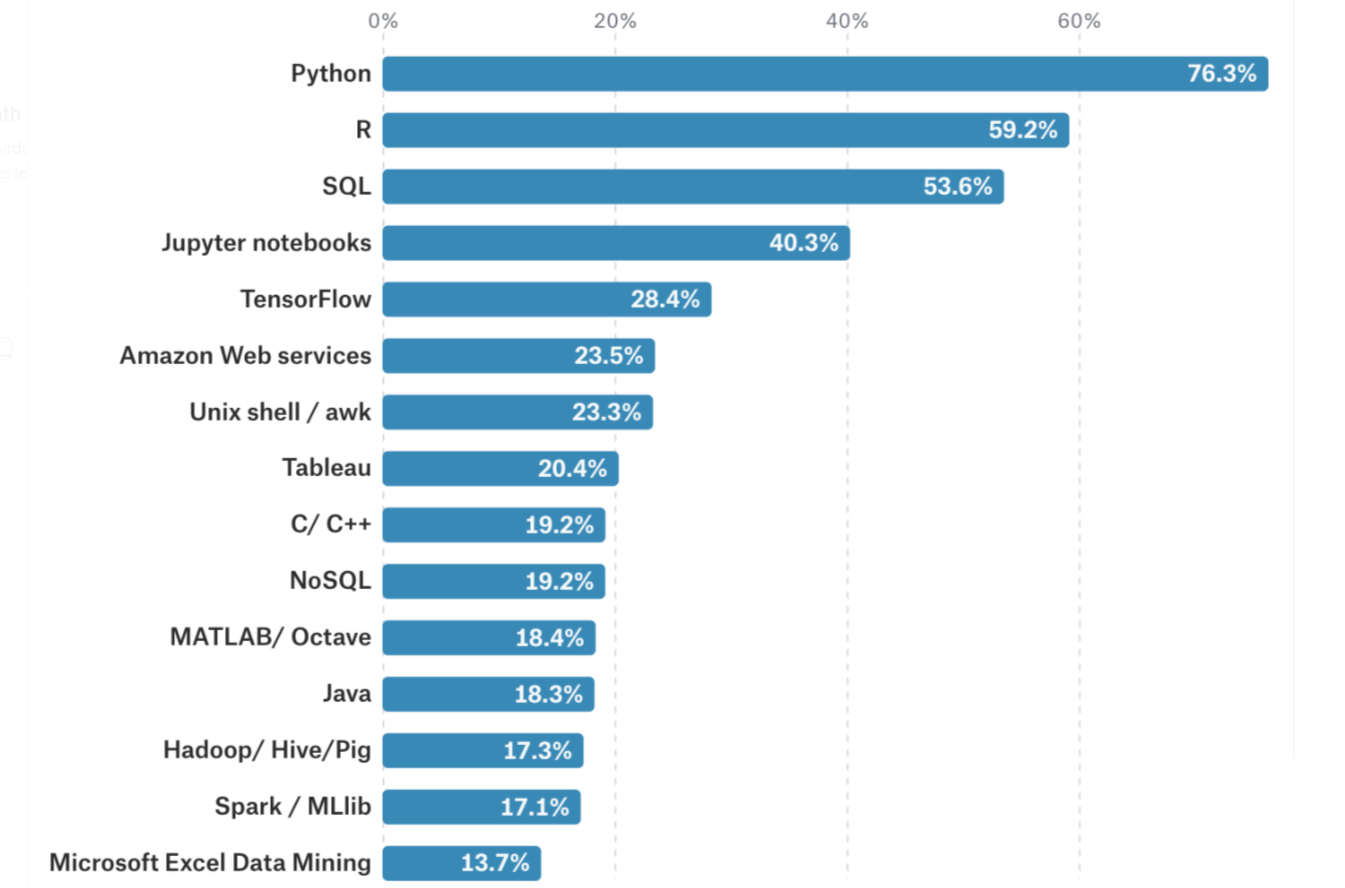
\includegraphics[width=0.9\linewidth,height=0.7\textheight]{imagem/linguagens} 

}

\caption{ }\label{fig:linguagens, figures-side}
\end{figure}

fonte:
\href{https://towardsdatascience.com/training-your-staff-in-data-science-heres-how-to-pick-the-right-programming-language-dda349354b18}{Towards
data science}

\hypertarget{data-literacy}{%
\section{Data Literacy}\label{data-literacy}}

\begin{figure}

{\centering 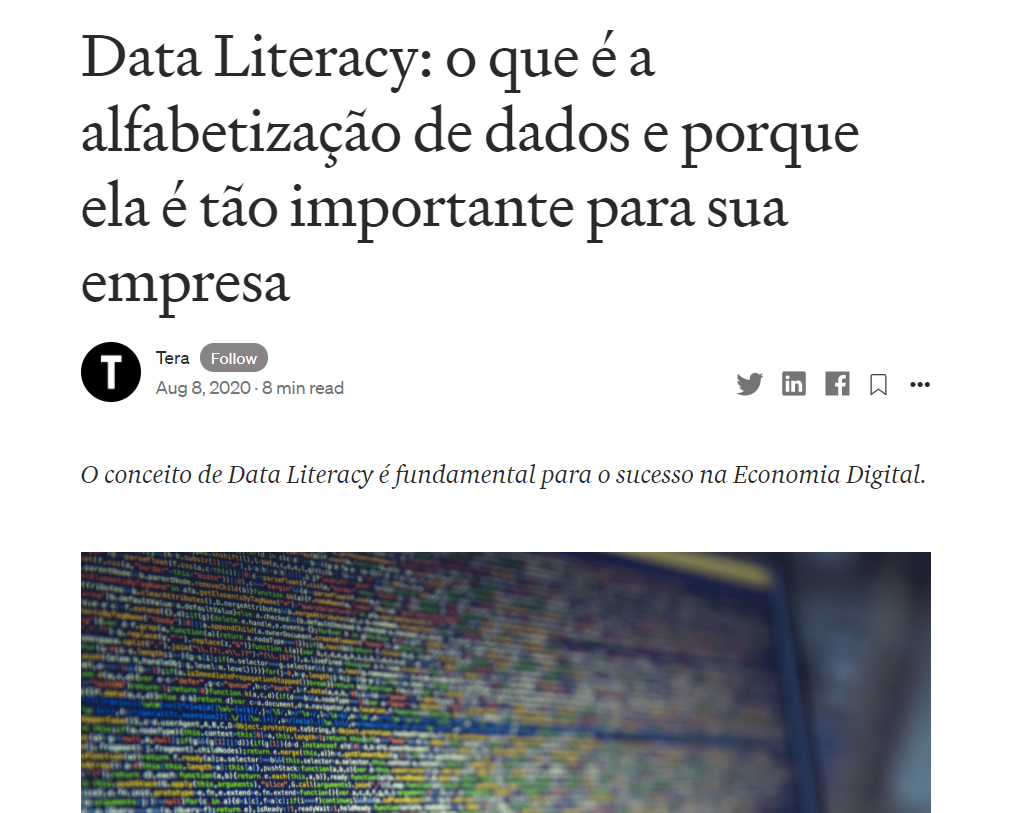
\includegraphics[width=0.7\linewidth,height=0.7\textheight]{imagem/data-literacy} 

}

\caption{ }\label{fig:literacy, figures-side}
\end{figure}

fonte:
\href{https://medium.com/somos-tera/data-literacy-o-que-\%C3\%A9-a-alfabetiza\%C3\%A7\%C3\%A3o-de-dados-e-porque-ela-\%C3\%A9-t\%C3\%A3o-importante-para-sua-empresa-951fcc5bcc67}{Medium}

\hypertarget{literatura-cientuxedfica}{%
\section{Literatura científica}\label{literatura-cientuxedfica}}

\begin{figure}

{\centering 
\includegraphics[width=1\linewidth,height=1\textheight]{imagem/analytics-capabilities} 

}

\caption{ }\label{fig:artigos, figures-side}
\end{figure}

\hypertarget{na-uxe1rea-de-empreendedorismo}{%
\section{Na área de
empreendedorismo}\label{na-uxe1rea-de-empreendedorismo}}

\begin{figure}

{\centering 
\includegraphics[width=0.8\linewidth,height=0.8\textheight]{imagem/sbe} 

}

\caption{ }\label{fig:sbe, figures-side}
\end{figure}

\hypertarget{o-r-uxe9-um-calculadora}{%
\section{O R é um calculadora}\label{o-r-uxe9-um-calculadora}}

\begin{Shaded}
\begin{Highlighting}[]
\CommentTok{# Operações básicas}
\DecValTok{5} \OperatorTok{+}\StringTok{ }\DecValTok{5}
\end{Highlighting}
\end{Shaded}

\begin{verbatim}
## [1] 10
\end{verbatim}

\begin{Shaded}
\begin{Highlighting}[]
\DecValTok{10} \OperatorTok{-}\StringTok{ }\DecValTok{6}
\end{Highlighting}
\end{Shaded}

\begin{verbatim}
## [1] 4
\end{verbatim}

\begin{Shaded}
\begin{Highlighting}[]
\DecValTok{10}\OperatorTok{*}\DecValTok{2}
\end{Highlighting}
\end{Shaded}

\begin{verbatim}
## [1] 20
\end{verbatim}

\begin{Shaded}
\begin{Highlighting}[]
\DecValTok{5}\OperatorTok{/}\DecValTok{2}
\end{Highlighting}
\end{Shaded}

\begin{verbatim}
## [1] 2.5
\end{verbatim}

\begin{Shaded}
\begin{Highlighting}[]
\DecValTok{5}\OperatorTok{**}\DecValTok{2}
\end{Highlighting}
\end{Shaded}

\begin{verbatim}
## [1] 25
\end{verbatim}

\hypertarget{operauxe7uxf5es-de-atribuiuxe7uxe3o}{%
\section{Operações de
atribuição}\label{operauxe7uxf5es-de-atribuiuxe7uxe3o}}

\begin{Shaded}
\begin{Highlighting}[]
\KeywordTok{sqrt}\NormalTok{(}\DecValTok{16}\NormalTok{)}
\end{Highlighting}
\end{Shaded}

\begin{verbatim}
## [1] 4
\end{verbatim}

\begin{Shaded}
\begin{Highlighting}[]
\DecValTok{5}\OperatorTok{*}\NormalTok{(}\DecValTok{50-45}\NormalTok{)}
\end{Highlighting}
\end{Shaded}

\begin{verbatim}
## [1] 25
\end{verbatim}

\begin{Shaded}
\begin{Highlighting}[]
\CommentTok{#Atribuições}
\NormalTok{x <-}\StringTok{ }\DecValTok{5} \OperatorTok{+}\StringTok{ }\DecValTok{5}
\NormalTok{y <-}\StringTok{ }\DecValTok{10} \OperatorTok{-}\StringTok{ }\DecValTok{16}
\NormalTok{a <-}\StringTok{ }\DecValTok{9}
\NormalTok{soma <-}\StringTok{ }\NormalTok{a }\OperatorTok{+}\StringTok{ }\NormalTok{x}
\NormalTok{nome <-}\StringTok{ "daniel"}
\NormalTok{certo <-}\StringTok{ }\OtherTok{TRUE}
\end{Highlighting}
\end{Shaded}

\hypertarget{operauxe7uxf5es-buxe1sicas}{%
\section{Operações básicas}\label{operauxe7uxf5es-buxe1sicas}}

\begin{Shaded}
\begin{Highlighting}[]
\NormalTok{pesoDaniel <-}\StringTok{ }\DecValTok{79}
\NormalTok{alturaDaniel <-}\StringTok{ }\FloatTok{1.78}
\NormalTok{imcDaniel <-}\StringTok{ }\NormalTok{pesoDaniel}\OperatorTok{/}\NormalTok{alturaDaniel}\OperatorTok{**}\DecValTok{2}
\end{Highlighting}
\end{Shaded}

Calcule o IMC de todas as pessoas

\begin{figure}

{\centering 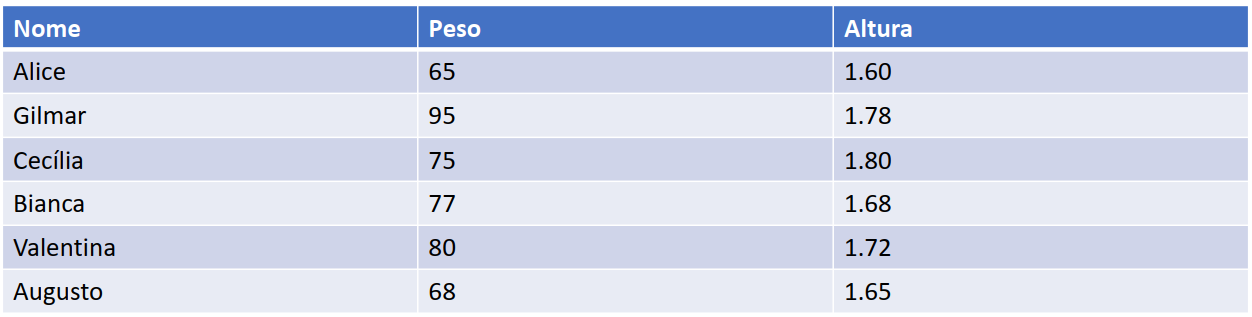
\includegraphics[width=0.9\linewidth,height=0.9\textheight]{imagem/imc} 

}

\caption{ }\label{fig:imc, figures-side}
\end{figure}

\hypertarget{vetores}{%
\section{Vetores}\label{vetores}}

Você até pode fazer o IMC de cada um individualmente.

Mas vou apresentar uma forma de resolver - existem várias formas, usando
função, loops - usando um tipo de objeto chamado \textbf{vetor}. O vetor
é um conjunto unidimensional de objetos de um mesmo tipo.

Traduzindo\ldots{} imagina uma tabela de excel formada por várias
colunas. Uma das colunas é a idade e está expressa em número. Pronto, um
vetor é como se fosse uma coluna com valores de um mesmo tipo.

\begin{Shaded}
\begin{Highlighting}[]
\CommentTok{# trabalhando com vetores}
\NormalTok{pesos <-}\StringTok{ }\KeywordTok{c}\NormalTok{(}\DecValTok{65}\NormalTok{, }\DecValTok{95}\NormalTok{, }\DecValTok{75}\NormalTok{, }\DecValTok{77}\NormalTok{, }\DecValTok{80}\NormalTok{, }\DecValTok{68}\NormalTok{)}
\NormalTok{alturas <-}\StringTok{ }\KeywordTok{c}\NormalTok{(}\FloatTok{1.60}\NormalTok{, }\FloatTok{1.78}\NormalTok{, }\FloatTok{1.80}\NormalTok{, }\FloatTok{1.68}\NormalTok{, }\FloatTok{1.72}\NormalTok{, }\FloatTok{1.65}\NormalTok{)}
\NormalTok{imc <-}\StringTok{ }\NormalTok{pesos}\OperatorTok{/}\NormalTok{alturas}\OperatorTok{**}\DecValTok{2}
\NormalTok{imc}
\end{Highlighting}
\end{Shaded}

\begin{verbatim}
## [1] 25.39062 29.98359 23.14815 27.28175 27.04164 24.97704
\end{verbatim}

\hypertarget{daniel-consigo-arredondar}{%
\section{Daniel, consigo arredondar?}\label{daniel-consigo-arredondar}}

Consegue!

\begin{Shaded}
\begin{Highlighting}[]
\KeywordTok{help}\NormalTok{(round)}
\KeywordTok{round}\NormalTok{(imc, }\DecValTok{2}\NormalTok{)}
\end{Highlighting}
\end{Shaded}

\begin{verbatim}
## [1] 25.39 29.98 23.15 27.28 27.04 24.98
\end{verbatim}

\begin{Shaded}
\begin{Highlighting}[]
\NormalTok{imc <-}\StringTok{ }\KeywordTok{round}\NormalTok{(imc, }\DecValTok{2}\NormalTok{) }\CommentTok{#estou sobrescrevendo um vetor}
\CommentTok{# arredondado sobre ele mesmo}
\NormalTok{imc}
\end{Highlighting}
\end{Shaded}

\begin{verbatim}
## [1] 25.39 29.98 23.15 27.28 27.04 24.98
\end{verbatim}

\hypertarget{matrizes}{%
\section{Matrizes}\label{matrizes}}

As \textbf{matrizes} possui uma estrutura tabular, com linhas e colunas.
Porém, semelhante ao vetor, todos os objetos devem ser de um mesmo tipo
(ex.: tudo número, tudo caracter).

\begin{Shaded}
\begin{Highlighting}[]
\NormalTok{Matriz<-}\KeywordTok{cbind}\NormalTok{(pesos,alturas,imc)}
\NormalTok{Matriz}
\end{Highlighting}
\end{Shaded}

\begin{verbatim}
##      pesos alturas   imc
## [1,]    65    1.60 25.39
## [2,]    95    1.78 29.98
## [3,]    75    1.80 23.15
## [4,]    77    1.68 27.28
## [5,]    80    1.72 27.04
## [6,]    68    1.65 24.98
\end{verbatim}

\hypertarget{matrizes-1}{%
\section{Matrizes}\label{matrizes-1}}

Veja que tem uma carinha de tabela. Mas daqui para frente vamos
trabalhar com outra estrutura chamada \textbf{dataframe}. Essa estrutura
tem formato tabular e ainda permite que os objetos tenham tipos
diferentes, ou seja, posso ter uma coluna numérica, outra no formato
data, outra no formato de caracteres e assim por diante.

Existe um tipo de estrutura de dados chamado \textbf{lista} muito
importante também. Mas entrar nele é assunto para um curso de R
intermediário.

\begin{Shaded}
\begin{Highlighting}[]
\KeywordTok{rownames}\NormalTok{(Matriz) <-}\StringTok{ }\KeywordTok{c}\NormalTok{(}\StringTok{"Alice"}\NormalTok{,}\StringTok{"Gilmar"}\NormalTok{,}\StringTok{"Cecilia"}\NormalTok{,}\StringTok{"Bianca"}\NormalTok{,}\StringTok{"Valentina"}\NormalTok{,}\StringTok{"Augusto"}\NormalTok{)}
\NormalTok{Matriz}
\end{Highlighting}
\end{Shaded}

\begin{verbatim}
##           pesos alturas   imc
## Alice        65    1.60 25.39
## Gilmar       95    1.78 29.98
## Cecilia      75    1.80 23.15
## Bianca       77    1.68 27.28
## Valentina    80    1.72 27.04
## Augusto      68    1.65 24.98
\end{verbatim}

\hypertarget{introduzindo-funuxe7uxf5es-para-manipulauxe7uxe3o-de-dados}{%
\section{Introduzindo funções para manipulação de
dados}\label{introduzindo-funuxe7uxf5es-para-manipulauxe7uxe3o-de-dados}}

\hypertarget{inspecionando-o-dataframe}{%
\section{Inspecionando o dataframe}\label{inspecionando-o-dataframe}}

\begin{Shaded}
\begin{Highlighting}[]
\KeywordTok{library}\NormalTok{(gapminder)}
\NormalTok{basePaises <-}\StringTok{ }\NormalTok{gapminder}

\CommentTok{# inspecionando a estrutura da base}
\KeywordTok{str}\NormalTok{(basePaises)}
\end{Highlighting}
\end{Shaded}

\begin{verbatim}
## tibble [1,704 x 6] (S3: tbl_df/tbl/data.frame)
##  $ country  : Factor w/ 142 levels "Afghanistan",..: 1 1 1 1 1 1 1 1 1 1 ...
##  $ continent: Factor w/ 5 levels "Africa","Americas",..: 3 3 3 3 3 3 3 3 3 3 ...
##  $ year     : int [1:1704] 1952 1957 1962 1967 1972 1977 1982 1987 1992 1997 ...
##  $ lifeExp  : num [1:1704] 28.8 30.3 32 34 36.1 ...
##  $ pop      : int [1:1704] 8425333 9240934 10267083 11537966 13079460 14880372 12881816 13867957 16317921 22227415 ...
##  $ gdpPercap: num [1:1704] 779 821 853 836 740 ...
\end{verbatim}

\hypertarget{inspecionando-elementos}{%
\section{Inspecionando elementos}\label{inspecionando-elementos}}

\begin{Shaded}
\begin{Highlighting}[]
\CommentTok{# inspecionando as 6 primeiras observações }
\KeywordTok{head}\NormalTok{(basePaises)}
\end{Highlighting}
\end{Shaded}

\begin{verbatim}
## # A tibble: 6 x 6
##   country     continent  year lifeExp      pop gdpPercap
##   <fct>       <fct>     <int>   <dbl>    <int>     <dbl>
## 1 Afghanistan Asia       1952    28.8  8425333      779.
## 2 Afghanistan Asia       1957    30.3  9240934      821.
## 3 Afghanistan Asia       1962    32.0 10267083      853.
## 4 Afghanistan Asia       1967    34.0 11537966      836.
## 5 Afghanistan Asia       1972    36.1 13079460      740.
## 6 Afghanistan Asia       1977    38.4 14880372      786.
\end{verbatim}

\hypertarget{inspecionando-elementos-1}{%
\section{Inspecionando elementos}\label{inspecionando-elementos-1}}

\begin{Shaded}
\begin{Highlighting}[]
\CommentTok{# inspecionando as 10 últimas observações}
\KeywordTok{tail}\NormalTok{(basePaises, }\DataTypeTok{n =} \DecValTok{10}\NormalTok{)}
\end{Highlighting}
\end{Shaded}

\begin{verbatim}
## # A tibble: 10 x 6
##    country  continent  year lifeExp      pop gdpPercap
##    <fct>    <fct>     <int>   <dbl>    <int>     <dbl>
##  1 Zimbabwe Africa     1962    52.4  4277736      527.
##  2 Zimbabwe Africa     1967    54.0  4995432      570.
##  3 Zimbabwe Africa     1972    55.6  5861135      799.
##  4 Zimbabwe Africa     1977    57.7  6642107      686.
##  5 Zimbabwe Africa     1982    60.4  7636524      789.
##  6 Zimbabwe Africa     1987    62.4  9216418      706.
##  7 Zimbabwe Africa     1992    60.4 10704340      693.
##  8 Zimbabwe Africa     1997    46.8 11404948      792.
##  9 Zimbabwe Africa     2002    40.0 11926563      672.
## 10 Zimbabwe Africa     2007    43.5 12311143      470.
\end{verbatim}

\hypertarget{inspecionando-elementos-2}{%
\section{Inspecionando elementos}\label{inspecionando-elementos-2}}

\begin{Shaded}
\begin{Highlighting}[]
\CommentTok{# estatísticas descritivas da base}
\KeywordTok{summary}\NormalTok{(basePaises)}
\end{Highlighting}
\end{Shaded}

\begin{verbatim}
##         country        continent        year         lifeExp     
##  Afghanistan:  12   Africa  :624   Min.   :1952   Min.   :23.60  
##  Albania    :  12   Americas:300   1st Qu.:1966   1st Qu.:48.20  
##  Algeria    :  12   Asia    :396   Median :1980   Median :60.71  
##  Angola     :  12   Europe  :360   Mean   :1980   Mean   :59.47  
##  Argentina  :  12   Oceania : 24   3rd Qu.:1993   3rd Qu.:70.85  
##  Australia  :  12                  Max.   :2007   Max.   :82.60  
##  (Other)    :1632                                                
##       pop              gdpPercap       
##  Min.   :6.001e+04   Min.   :   241.2  
##  1st Qu.:2.794e+06   1st Qu.:  1202.1  
##  Median :7.024e+06   Median :  3531.8  
##  Mean   :2.960e+07   Mean   :  7215.3  
##  3rd Qu.:1.959e+07   3rd Qu.:  9325.5  
##  Max.   :1.319e+09   Max.   :113523.1  
## 
\end{verbatim}

\hypertarget{inspecionando-elementos-3}{%
\section{Inspecionando elementos}\label{inspecionando-elementos-3}}

\begin{Shaded}
\begin{Highlighting}[]
\CommentTok{# Acessando uma variável da base}
\NormalTok{basePaises}\OperatorTok{$}\NormalTok{continent}
\end{Highlighting}
\end{Shaded}

\begin{verbatim}
##    [1] Asia     Asia     Asia     Asia     Asia     Asia     Asia     Asia    
##    [9] Asia     Asia     Asia     Asia     Europe   Europe   Europe   Europe  
##   [17] Europe   Europe   Europe   Europe   Europe   Europe   Europe   Europe  
##   [25] Africa   Africa   Africa   Africa   Africa   Africa   Africa   Africa  
##   [33] Africa   Africa   Africa   Africa   Africa   Africa   Africa   Africa  
##   [41] Africa   Africa   Africa   Africa   Africa   Africa   Africa   Africa  
##   [49] Americas Americas Americas Americas Americas Americas Americas Americas
##   [57] Americas Americas Americas Americas Oceania  Oceania  Oceania  Oceania 
##   [65] Oceania  Oceania  Oceania  Oceania  Oceania  Oceania  Oceania  Oceania 
##   [73] Europe   Europe   Europe   Europe   Europe   Europe   Europe   Europe  
##   [81] Europe   Europe   Europe   Europe   Asia     Asia     Asia     Asia    
##   [89] Asia     Asia     Asia     Asia     Asia     Asia     Asia     Asia    
##   [97] Asia     Asia     Asia     Asia     Asia     Asia     Asia     Asia    
##  [105] Asia     Asia     Asia     Asia     Europe   Europe   Europe   Europe  
##  [113] Europe   Europe   Europe   Europe   Europe   Europe   Europe   Europe  
##  [121] Africa   Africa   Africa   Africa   Africa   Africa   Africa   Africa  
##  [129] Africa   Africa   Africa   Africa   Americas Americas Americas Americas
##  [137] Americas Americas Americas Americas Americas Americas Americas Americas
##  [145] Europe   Europe   Europe   Europe   Europe   Europe   Europe   Europe  
##  [153] Europe   Europe   Europe   Europe   Africa   Africa   Africa   Africa  
##  [161] Africa   Africa   Africa   Africa   Africa   Africa   Africa   Africa  
##  [169] Americas Americas Americas Americas Americas Americas Americas Americas
##  [177] Americas Americas Americas Americas Europe   Europe   Europe   Europe  
##  [185] Europe   Europe   Europe   Europe   Europe   Europe   Europe   Europe  
##  [193] Africa   Africa   Africa   Africa   Africa   Africa   Africa   Africa  
##  [201] Africa   Africa   Africa   Africa   Africa   Africa   Africa   Africa  
##  [209] Africa   Africa   Africa   Africa   Africa   Africa   Africa   Africa  
##  [217] Asia     Asia     Asia     Asia     Asia     Asia     Asia     Asia    
##  [225] Asia     Asia     Asia     Asia     Africa   Africa   Africa   Africa  
##  [233] Africa   Africa   Africa   Africa   Africa   Africa   Africa   Africa  
##  [241] Americas Americas Americas Americas Americas Americas Americas Americas
##  [249] Americas Americas Americas Americas Africa   Africa   Africa   Africa  
##  [257] Africa   Africa   Africa   Africa   Africa   Africa   Africa   Africa  
##  [265] Africa   Africa   Africa   Africa   Africa   Africa   Africa   Africa  
##  [273] Africa   Africa   Africa   Africa   Americas Americas Americas Americas
##  [281] Americas Americas Americas Americas Americas Americas Americas Americas
##  [289] Asia     Asia     Asia     Asia     Asia     Asia     Asia     Asia    
##  [297] Asia     Asia     Asia     Asia     Americas Americas Americas Americas
##  [305] Americas Americas Americas Americas Americas Americas Americas Americas
##  [313] Africa   Africa   Africa   Africa   Africa   Africa   Africa   Africa  
##  [321] Africa   Africa   Africa   Africa   Africa   Africa   Africa   Africa  
##  [329] Africa   Africa   Africa   Africa   Africa   Africa   Africa   Africa  
##  [337] Africa   Africa   Africa   Africa   Africa   Africa   Africa   Africa  
##  [345] Africa   Africa   Africa   Africa   Americas Americas Americas Americas
##  [353] Americas Americas Americas Americas Americas Americas Americas Americas
##  [361] Africa   Africa   Africa   Africa   Africa   Africa   Africa   Africa  
##  [369] Africa   Africa   Africa   Africa   Europe   Europe   Europe   Europe  
##  [377] Europe   Europe   Europe   Europe   Europe   Europe   Europe   Europe  
##  [385] Americas Americas Americas Americas Americas Americas Americas Americas
##  [393] Americas Americas Americas Americas Europe   Europe   Europe   Europe  
##  [401] Europe   Europe   Europe   Europe   Europe   Europe   Europe   Europe  
##  [409] Europe   Europe   Europe   Europe   Europe   Europe   Europe   Europe  
##  [417] Europe   Europe   Europe   Europe   Africa   Africa   Africa   Africa  
##  [425] Africa   Africa   Africa   Africa   Africa   Africa   Africa   Africa  
##  [433] Americas Americas Americas Americas Americas Americas Americas Americas
##  [441] Americas Americas Americas Americas Americas Americas Americas Americas
##  [449] Americas Americas Americas Americas Americas Americas Americas Americas
##  [457] Africa   Africa   Africa   Africa   Africa   Africa   Africa   Africa  
##  [465] Africa   Africa   Africa   Africa   Americas Americas Americas Americas
##  [473] Americas Americas Americas Americas Americas Americas Americas Americas
##  [481] Africa   Africa   Africa   Africa   Africa   Africa   Africa   Africa  
##  [489] Africa   Africa   Africa   Africa   Africa   Africa   Africa   Africa  
##  [497] Africa   Africa   Africa   Africa   Africa   Africa   Africa   Africa  
##  [505] Africa   Africa   Africa   Africa   Africa   Africa   Africa   Africa  
##  [513] Africa   Africa   Africa   Africa   Europe   Europe   Europe   Europe  
##  [521] Europe   Europe   Europe   Europe   Europe   Europe   Europe   Europe  
##  [529] Europe   Europe   Europe   Europe   Europe   Europe   Europe   Europe  
##  [537] Europe   Europe   Europe   Europe   Africa   Africa   Africa   Africa  
##  [545] Africa   Africa   Africa   Africa   Africa   Africa   Africa   Africa  
##  [553] Africa   Africa   Africa   Africa   Africa   Africa   Africa   Africa  
##  [561] Africa   Africa   Africa   Africa   Europe   Europe   Europe   Europe  
##  [569] Europe   Europe   Europe   Europe   Europe   Europe   Europe   Europe  
##  [577] Africa   Africa   Africa   Africa   Africa   Africa   Africa   Africa  
##  [585] Africa   Africa   Africa   Africa   Europe   Europe   Europe   Europe  
##  [593] Europe   Europe   Europe   Europe   Europe   Europe   Europe   Europe  
##  [601] Americas Americas Americas Americas Americas Americas Americas Americas
##  [609] Americas Americas Americas Americas Africa   Africa   Africa   Africa  
##  [617] Africa   Africa   Africa   Africa   Africa   Africa   Africa   Africa  
##  [625] Africa   Africa   Africa   Africa   Africa   Africa   Africa   Africa  
##  [633] Africa   Africa   Africa   Africa   Americas Americas Americas Americas
##  [641] Americas Americas Americas Americas Americas Americas Americas Americas
##  [649] Americas Americas Americas Americas Americas Americas Americas Americas
##  [657] Americas Americas Americas Americas Asia     Asia     Asia     Asia    
##  [665] Asia     Asia     Asia     Asia     Asia     Asia     Asia     Asia    
##  [673] Europe   Europe   Europe   Europe   Europe   Europe   Europe   Europe  
##  [681] Europe   Europe   Europe   Europe   Europe   Europe   Europe   Europe  
##  [689] Europe   Europe   Europe   Europe   Europe   Europe   Europe   Europe  
##  [697] Asia     Asia     Asia     Asia     Asia     Asia     Asia     Asia    
##  [705] Asia     Asia     Asia     Asia     Asia     Asia     Asia     Asia    
##  [713] Asia     Asia     Asia     Asia     Asia     Asia     Asia     Asia    
##  [721] Asia     Asia     Asia     Asia     Asia     Asia     Asia     Asia    
##  [729] Asia     Asia     Asia     Asia     Asia     Asia     Asia     Asia    
##  [737] Asia     Asia     Asia     Asia     Asia     Asia     Asia     Asia    
##  [745] Europe   Europe   Europe   Europe   Europe   Europe   Europe   Europe  
##  [753] Europe   Europe   Europe   Europe   Asia     Asia     Asia     Asia    
##  [761] Asia     Asia     Asia     Asia     Asia     Asia     Asia     Asia    
##  [769] Europe   Europe   Europe   Europe   Europe   Europe   Europe   Europe  
##  [777] Europe   Europe   Europe   Europe   Americas Americas Americas Americas
##  [785] Americas Americas Americas Americas Americas Americas Americas Americas
##  [793] Asia     Asia     Asia     Asia     Asia     Asia     Asia     Asia    
##  [801] Asia     Asia     Asia     Asia     Asia     Asia     Asia     Asia    
##  [809] Asia     Asia     Asia     Asia     Asia     Asia     Asia     Asia    
##  [817] Africa   Africa   Africa   Africa   Africa   Africa   Africa   Africa  
##  [825] Africa   Africa   Africa   Africa   Asia     Asia     Asia     Asia    
##  [833] Asia     Asia     Asia     Asia     Asia     Asia     Asia     Asia    
##  [841] Asia     Asia     Asia     Asia     Asia     Asia     Asia     Asia    
##  [849] Asia     Asia     Asia     Asia     Asia     Asia     Asia     Asia    
##  [857] Asia     Asia     Asia     Asia     Asia     Asia     Asia     Asia    
##  [865] Asia     Asia     Asia     Asia     Asia     Asia     Asia     Asia    
##  [873] Asia     Asia     Asia     Asia     Africa   Africa   Africa   Africa  
##  [881] Africa   Africa   Africa   Africa   Africa   Africa   Africa   Africa  
##  [889] Africa   Africa   Africa   Africa   Africa   Africa   Africa   Africa  
##  [897] Africa   Africa   Africa   Africa   Africa   Africa   Africa   Africa  
##  [905] Africa   Africa   Africa   Africa   Africa   Africa   Africa   Africa  
##  [913] Africa   Africa   Africa   Africa   Africa   Africa   Africa   Africa  
##  [921] Africa   Africa   Africa   Africa   Africa   Africa   Africa   Africa  
##  [929] Africa   Africa   Africa   Africa   Africa   Africa   Africa   Africa  
##  [937] Asia     Asia     Asia     Asia     Asia     Asia     Asia     Asia    
##  [945] Asia     Asia     Asia     Asia     Africa   Africa   Africa   Africa  
##  [953] Africa   Africa   Africa   Africa   Africa   Africa   Africa   Africa  
##  [961] Africa   Africa   Africa   Africa   Africa   Africa   Africa   Africa  
##  [969] Africa   Africa   Africa   Africa   Africa   Africa   Africa   Africa  
##  [977] Africa   Africa   Africa   Africa   Africa   Africa   Africa   Africa  
##  [985] Americas Americas Americas Americas Americas Americas Americas Americas
##  [993] Americas Americas Americas Americas Asia     Asia     Asia     Asia    
## [1001] Asia     Asia     Asia     Asia     Asia     Asia     Asia     Asia    
## [1009] Europe   Europe   Europe   Europe   Europe   Europe   Europe   Europe  
## [1017] Europe   Europe   Europe   Europe   Africa   Africa   Africa   Africa  
## [1025] Africa   Africa   Africa   Africa   Africa   Africa   Africa   Africa  
## [1033] Africa   Africa   Africa   Africa   Africa   Africa   Africa   Africa  
## [1041] Africa   Africa   Africa   Africa   Asia     Asia     Asia     Asia    
## [1049] Asia     Asia     Asia     Asia     Asia     Asia     Asia     Asia    
## [1057] Africa   Africa   Africa   Africa   Africa   Africa   Africa   Africa  
## [1065] Africa   Africa   Africa   Africa   Asia     Asia     Asia     Asia    
## [1073] Asia     Asia     Asia     Asia     Asia     Asia     Asia     Asia    
## [1081] Europe   Europe   Europe   Europe   Europe   Europe   Europe   Europe  
## [1089] Europe   Europe   Europe   Europe   Oceania  Oceania  Oceania  Oceania 
## [1097] Oceania  Oceania  Oceania  Oceania  Oceania  Oceania  Oceania  Oceania 
## [1105] Americas Americas Americas Americas Americas Americas Americas Americas
## [1113] Americas Americas Americas Americas Africa   Africa   Africa   Africa  
## [1121] Africa   Africa   Africa   Africa   Africa   Africa   Africa   Africa  
## [1129] Africa   Africa   Africa   Africa   Africa   Africa   Africa   Africa  
## [1137] Africa   Africa   Africa   Africa   Europe   Europe   Europe   Europe  
## [1145] Europe   Europe   Europe   Europe   Europe   Europe   Europe   Europe  
## [1153] Asia     Asia     Asia     Asia     Asia     Asia     Asia     Asia    
## [1161] Asia     Asia     Asia     Asia     Asia     Asia     Asia     Asia    
## [1169] Asia     Asia     Asia     Asia     Asia     Asia     Asia     Asia    
## [1177] Americas Americas Americas Americas Americas Americas Americas Americas
## [1185] Americas Americas Americas Americas Americas Americas Americas Americas
## [1193] Americas Americas Americas Americas Americas Americas Americas Americas
## [1201] Americas Americas Americas Americas Americas Americas Americas Americas
## [1209] Americas Americas Americas Americas Asia     Asia     Asia     Asia    
## [1217] Asia     Asia     Asia     Asia     Asia     Asia     Asia     Asia    
## [1225] Europe   Europe   Europe   Europe   Europe   Europe   Europe   Europe  
## [1233] Europe   Europe   Europe   Europe   Europe   Europe   Europe   Europe  
## [1241] Europe   Europe   Europe   Europe   Europe   Europe   Europe   Europe  
## [1249] Americas Americas Americas Americas Americas Americas Americas Americas
## [1257] Americas Americas Americas Americas Africa   Africa   Africa   Africa  
## [1265] Africa   Africa   Africa   Africa   Africa   Africa   Africa   Africa  
## [1273] Europe   Europe   Europe   Europe   Europe   Europe   Europe   Europe  
## [1281] Europe   Europe   Europe   Europe   Africa   Africa   Africa   Africa  
## [1289] Africa   Africa   Africa   Africa   Africa   Africa   Africa   Africa  
## [1297] Africa   Africa   Africa   Africa   Africa   Africa   Africa   Africa  
## [1305] Africa   Africa   Africa   Africa   Asia     Asia     Asia     Asia    
## [1313] Asia     Asia     Asia     Asia     Asia     Asia     Asia     Asia    
## [1321] Africa   Africa   Africa   Africa   Africa   Africa   Africa   Africa  
## [1329] Africa   Africa   Africa   Africa   Europe   Europe   Europe   Europe  
## [1337] Europe   Europe   Europe   Europe   Europe   Europe   Europe   Europe  
## [1345] Africa   Africa   Africa   Africa   Africa   Africa   Africa   Africa  
## [1353] Africa   Africa   Africa   Africa   Asia     Asia     Asia     Asia    
## [1361] Asia     Asia     Asia     Asia     Asia     Asia     Asia     Asia    
## [1369] Europe   Europe   Europe   Europe   Europe   Europe   Europe   Europe  
## [1377] Europe   Europe   Europe   Europe   Europe   Europe   Europe   Europe  
## [1385] Europe   Europe   Europe   Europe   Europe   Europe   Europe   Europe  
## [1393] Africa   Africa   Africa   Africa   Africa   Africa   Africa   Africa  
## [1401] Africa   Africa   Africa   Africa   Africa   Africa   Africa   Africa  
## [1409] Africa   Africa   Africa   Africa   Africa   Africa   Africa   Africa  
## [1417] Europe   Europe   Europe   Europe   Europe   Europe   Europe   Europe  
## [1425] Europe   Europe   Europe   Europe   Asia     Asia     Asia     Asia    
## [1433] Asia     Asia     Asia     Asia     Asia     Asia     Asia     Asia    
## [1441] Africa   Africa   Africa   Africa   Africa   Africa   Africa   Africa  
## [1449] Africa   Africa   Africa   Africa   Africa   Africa   Africa   Africa  
## [1457] Africa   Africa   Africa   Africa   Africa   Africa   Africa   Africa  
## [1465] Europe   Europe   Europe   Europe   Europe   Europe   Europe   Europe  
## [1473] Europe   Europe   Europe   Europe   Europe   Europe   Europe   Europe  
## [1481] Europe   Europe   Europe   Europe   Europe   Europe   Europe   Europe  
## [1489] Asia     Asia     Asia     Asia     Asia     Asia     Asia     Asia    
## [1497] Asia     Asia     Asia     Asia     Asia     Asia     Asia     Asia    
## [1505] Asia     Asia     Asia     Asia     Asia     Asia     Asia     Asia    
## [1513] Africa   Africa   Africa   Africa   Africa   Africa   Africa   Africa  
## [1521] Africa   Africa   Africa   Africa   Asia     Asia     Asia     Asia    
## [1529] Asia     Asia     Asia     Asia     Asia     Asia     Asia     Asia    
## [1537] Africa   Africa   Africa   Africa   Africa   Africa   Africa   Africa  
## [1545] Africa   Africa   Africa   Africa   Americas Americas Americas Americas
## [1553] Americas Americas Americas Americas Americas Americas Americas Americas
## [1561] Africa   Africa   Africa   Africa   Africa   Africa   Africa   Africa  
## [1569] Africa   Africa   Africa   Africa   Europe   Europe   Europe   Europe  
## [1577] Europe   Europe   Europe   Europe   Europe   Europe   Europe   Europe  
## [1585] Africa   Africa   Africa   Africa   Africa   Africa   Africa   Africa  
## [1593] Africa   Africa   Africa   Africa   Europe   Europe   Europe   Europe  
## [1601] Europe   Europe   Europe   Europe   Europe   Europe   Europe   Europe  
## [1609] Americas Americas Americas Americas Americas Americas Americas Americas
## [1617] Americas Americas Americas Americas Americas Americas Americas Americas
## [1625] Americas Americas Americas Americas Americas Americas Americas Americas
## [1633] Americas Americas Americas Americas Americas Americas Americas Americas
## [1641] Americas Americas Americas Americas Asia     Asia     Asia     Asia    
## [1649] Asia     Asia     Asia     Asia     Asia     Asia     Asia     Asia    
## [1657] Asia     Asia     Asia     Asia     Asia     Asia     Asia     Asia    
## [1665] Asia     Asia     Asia     Asia     Asia     Asia     Asia     Asia    
## [1673] Asia     Asia     Asia     Asia     Asia     Asia     Asia     Asia    
## [1681] Africa   Africa   Africa   Africa   Africa   Africa   Africa   Africa  
## [1689] Africa   Africa   Africa   Africa   Africa   Africa   Africa   Africa  
## [1697] Africa   Africa   Africa   Africa   Africa   Africa   Africa   Africa  
## Levels: Africa Americas Asia Europe Oceania
\end{verbatim}

\hypertarget{inspecionando-elementos-4}{%
\section{Inspecionando elementos}\label{inspecionando-elementos-4}}

\begin{Shaded}
\begin{Highlighting}[]
\CommentTok{# Acessando elementos únicos}
\KeywordTok{unique}\NormalTok{(basePaises}\OperatorTok{$}\NormalTok{year)}
\end{Highlighting}
\end{Shaded}

\begin{verbatim}
##  [1] 1952 1957 1962 1967 1972 1977 1982 1987 1992 1997 2002 2007
\end{verbatim}

\begin{Shaded}
\begin{Highlighting}[]
\KeywordTok{mean}\NormalTok{(basePaises}\OperatorTok{$}\NormalTok{lifeExp)}
\end{Highlighting}
\end{Shaded}

\begin{verbatim}
## [1] 59.47444
\end{verbatim}

\begin{Shaded}
\begin{Highlighting}[]
\CommentTok{# Vamos instalar nosso primeiro pacote: dplyr}

\KeywordTok{library}\NormalTok{(dplyr)}
\KeywordTok{glimpse}\NormalTok{(basePaises)}
\end{Highlighting}
\end{Shaded}

\begin{verbatim}
## Rows: 1,704
## Columns: 6
## $ country   <fct> "Afghanistan", "Afghanistan", "Afghanistan", "Afghanistan", ~
## $ continent <fct> Asia, Asia, Asia, Asia, Asia, Asia, Asia, Asia, Asia, Asia, ~
## $ year      <int> 1952, 1957, 1962, 1967, 1972, 1977, 1982, 1987, 1992, 1997, ~
## $ lifeExp   <dbl> 28.801, 30.332, 31.997, 34.020, 36.088, 38.438, 39.854, 40.8~
## $ pop       <int> 8425333, 9240934, 10267083, 11537966, 13079460, 14880372, 12~
## $ gdpPercap <dbl> 779.4453, 820.8530, 853.1007, 836.1971, 739.9811, 786.1134, ~
\end{verbatim}

\hypertarget{abrindo-um-paruxeantese}{%
\section{Abrindo um parêntese}\label{abrindo-um-paruxeantese}}

\begin{figure}

{\centering 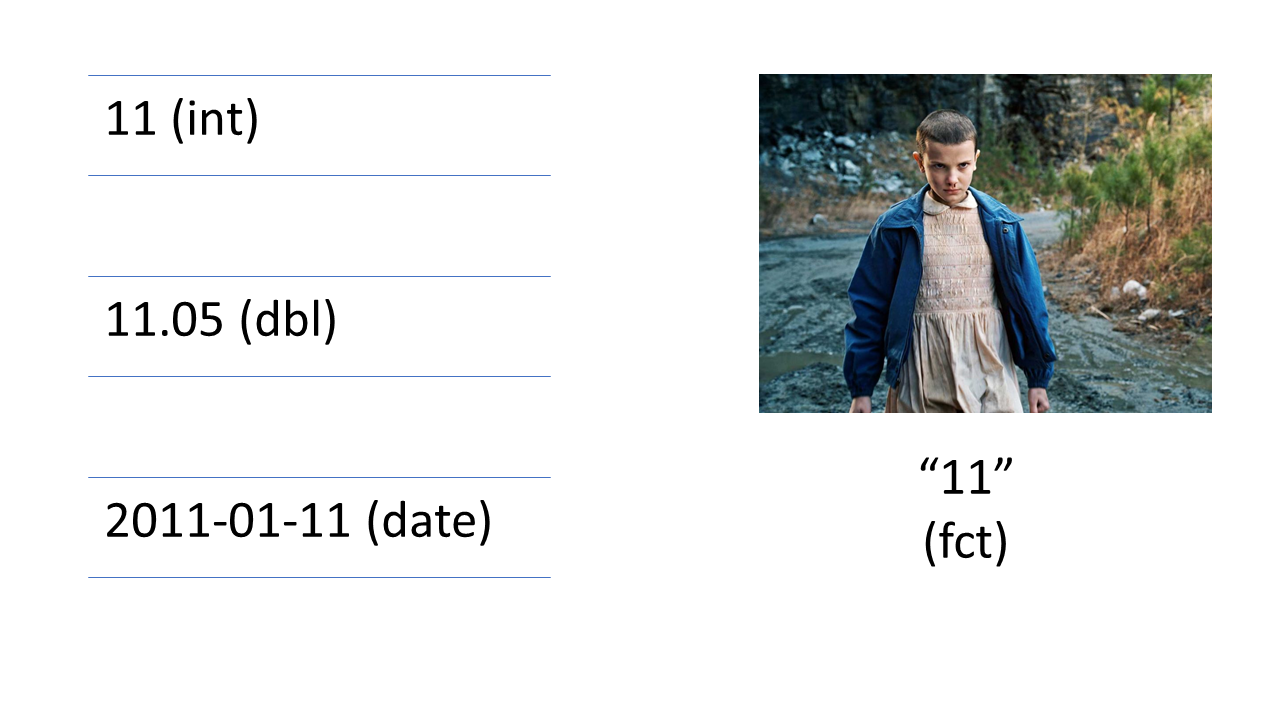
\includegraphics[width=1\linewidth,height=1\textheight]{imagem/eleven} 

}

\caption{ }\label{fig:eleven, figures-side}
\end{figure}

\hypertarget{funuxe7uxe3o-filter}{%
\section{Função filter}\label{funuxe7uxe3o-filter}}

\begin{Shaded}
\begin{Highlighting}[]
\NormalTok{basePaises }\OperatorTok\StringTok{ }
\StringTok{  }\KeywordTok{filter}\NormalTok{(continent }\OperatorTok{==}\StringTok{ "Asia"}\NormalTok{)}
\end{Highlighting}
\end{Shaded}

\begin{verbatim}
## # A tibble: 396 x 6
##    country     continent  year lifeExp      pop gdpPercap
##    <fct>       <fct>     <int>   <dbl>    <int>     <dbl>
##  1 Afghanistan Asia       1952    28.8  8425333      779.
##  2 Afghanistan Asia       1957    30.3  9240934      821.
##  3 Afghanistan Asia       1962    32.0 10267083      853.
##  4 Afghanistan Asia       1967    34.0 11537966      836.
##  5 Afghanistan Asia       1972    36.1 13079460      740.
##  6 Afghanistan Asia       1977    38.4 14880372      786.
##  7 Afghanistan Asia       1982    39.9 12881816      978.
##  8 Afghanistan Asia       1987    40.8 13867957      852.
##  9 Afghanistan Asia       1992    41.7 16317921      649.
## 10 Afghanistan Asia       1997    41.8 22227415      635.
## # ... with 386 more rows
\end{verbatim}

\hypertarget{funuxe7uxe3o-filter-1}{%
\section{Função filter}\label{funuxe7uxe3o-filter-1}}

\begin{Shaded}
\begin{Highlighting}[]
\NormalTok{basePaises}\OperatorTok
\StringTok{  }\KeywordTok{filter}\NormalTok{(continent }\OperatorTok{==}\StringTok{ "Americas"} \OperatorTok{&}\StringTok{ }\NormalTok{year}\OperatorTok{>}\DecValTok{1990}\NormalTok{)}
\end{Highlighting}
\end{Shaded}

\begin{verbatim}
## # A tibble: 100 x 6
##    country   continent  year lifeExp       pop gdpPercap
##    <fct>     <fct>     <int>   <dbl>     <int>     <dbl>
##  1 Argentina Americas   1992    71.9  33958947     9308.
##  2 Argentina Americas   1997    73.3  36203463    10967.
##  3 Argentina Americas   2002    74.3  38331121     8798.
##  4 Argentina Americas   2007    75.3  40301927    12779.
##  5 Bolivia   Americas   1992    60.0   6893451     2962.
##  6 Bolivia   Americas   1997    62.0   7693188     3326.
##  7 Bolivia   Americas   2002    63.9   8445134     3413.
##  8 Bolivia   Americas   2007    65.6   9119152     3822.
##  9 Brazil    Americas   1992    67.1 155975974     6950.
## 10 Brazil    Americas   1997    69.4 168546719     7958.
## # ... with 90 more rows
\end{verbatim}

\hypertarget{funuxe7uxe3o-filter-2}{%
\section{Função filter}\label{funuxe7uxe3o-filter-2}}

\begin{Shaded}
\begin{Highlighting}[]
\CommentTok{# != diferente }
\NormalTok{basePaises}\OperatorTok
\StringTok{  }\KeywordTok{filter}\NormalTok{(continent }\OperatorTok{!=}\StringTok{ "Oceania"}\NormalTok{)}
\end{Highlighting}
\end{Shaded}

\begin{verbatim}
## # A tibble: 1,680 x 6
##    country     continent  year lifeExp      pop gdpPercap
##    <fct>       <fct>     <int>   <dbl>    <int>     <dbl>
##  1 Afghanistan Asia       1952    28.8  8425333      779.
##  2 Afghanistan Asia       1957    30.3  9240934      821.
##  3 Afghanistan Asia       1962    32.0 10267083      853.
##  4 Afghanistan Asia       1967    34.0 11537966      836.
##  5 Afghanistan Asia       1972    36.1 13079460      740.
##  6 Afghanistan Asia       1977    38.4 14880372      786.
##  7 Afghanistan Asia       1982    39.9 12881816      978.
##  8 Afghanistan Asia       1987    40.8 13867957      852.
##  9 Afghanistan Asia       1992    41.7 16317921      649.
## 10 Afghanistan Asia       1997    41.8 22227415      635.
## # ... with 1,670 more rows
\end{verbatim}

\begin{Shaded}
\begin{Highlighting}[]
\CommentTok{# Você pode armazenar sua consulta em outro objeto}
\NormalTok{baseAsia <-}\StringTok{ }\NormalTok{basePaises}\OperatorTok
\StringTok{  }\KeywordTok{filter}\NormalTok{(continent }\OperatorTok{==}\StringTok{ "Asia"}\NormalTok{)}
\end{Highlighting}
\end{Shaded}

\hypertarget{funuxe7uxe3o-select}{%
\section{Função select}\label{funuxe7uxe3o-select}}

\begin{Shaded}
\begin{Highlighting}[]
\NormalTok{basePaises}\OperatorTok
\StringTok{  }\KeywordTok{select}\NormalTok{(year,country,gdpPercap)}
\end{Highlighting}
\end{Shaded}

\begin{verbatim}
## # A tibble: 1,704 x 3
##     year country     gdpPercap
##    <int> <fct>           <dbl>
##  1  1952 Afghanistan      779.
##  2  1957 Afghanistan      821.
##  3  1962 Afghanistan      853.
##  4  1967 Afghanistan      836.
##  5  1972 Afghanistan      740.
##  6  1977 Afghanistan      786.
##  7  1982 Afghanistan      978.
##  8  1987 Afghanistan      852.
##  9  1992 Afghanistan      649.
## 10  1997 Afghanistan      635.
## # ... with 1,694 more rows
\end{verbatim}

\hypertarget{funuxe7uxe3o-select-1}{%
\section{Função select}\label{funuxe7uxe3o-select-1}}

\begin{Shaded}
\begin{Highlighting}[]
\NormalTok{basePaises}\OperatorTok
\StringTok{  }\KeywordTok{select}\NormalTok{(}\OperatorTok{-}\NormalTok{lifeExp)}
\end{Highlighting}
\end{Shaded}

\begin{verbatim}
## # A tibble: 1,704 x 5
##    country     continent  year      pop gdpPercap
##    <fct>       <fct>     <int>    <int>     <dbl>
##  1 Afghanistan Asia       1952  8425333      779.
##  2 Afghanistan Asia       1957  9240934      821.
##  3 Afghanistan Asia       1962 10267083      853.
##  4 Afghanistan Asia       1967 11537966      836.
##  5 Afghanistan Asia       1972 13079460      740.
##  6 Afghanistan Asia       1977 14880372      786.
##  7 Afghanistan Asia       1982 12881816      978.
##  8 Afghanistan Asia       1987 13867957      852.
##  9 Afghanistan Asia       1992 16317921      649.
## 10 Afghanistan Asia       1997 22227415      635.
## # ... with 1,694 more rows
\end{verbatim}

\hypertarget{funuxe7uxe3o-select-filter}{%
\section{Função select + filter}\label{funuxe7uxe3o-select-filter}}

\begin{Shaded}
\begin{Highlighting}[]
\NormalTok{basePaises }\OperatorTok
\StringTok{  }\KeywordTok{filter}\NormalTok{(continent }\OperatorTok{==}\StringTok{ "Americas"} \OperatorTok{&}\StringTok{ }\NormalTok{year}\OperatorTok{>}\DecValTok{1990}\NormalTok{) }\OperatorTok
\StringTok{  }\KeywordTok{select}\NormalTok{(year,country,gdpPercap)}
\end{Highlighting}
\end{Shaded}

\begin{verbatim}
## # A tibble: 100 x 3
##     year country   gdpPercap
##    <int> <fct>         <dbl>
##  1  1992 Argentina     9308.
##  2  1997 Argentina    10967.
##  3  2002 Argentina     8798.
##  4  2007 Argentina    12779.
##  5  1992 Bolivia       2962.
##  6  1997 Bolivia       3326.
##  7  2002 Bolivia       3413.
##  8  2007 Bolivia       3822.
##  9  1992 Brazil        6950.
## 10  1997 Brazil        7958.
## # ... with 90 more rows
\end{verbatim}

\hypertarget{funuxe7uxe3o-mutate}{%
\section{Função mutate}\label{funuxe7uxe3o-mutate}}

Serve para criar uma nova variável

\begin{Shaded}
\begin{Highlighting}[]
\NormalTok{basePaises <-}\StringTok{ }\NormalTok{basePaises }\OperatorTok
\StringTok{  }\KeywordTok{mutate}\NormalTok{(}\DataTypeTok{GDP =}\NormalTok{ gdpPercap }\OperatorTok{*}\StringTok{ }\NormalTok{pop)}

\NormalTok{basePorte <-}\StringTok{ }\NormalTok{basePaises }\OperatorTok
\StringTok{  }\KeywordTok{filter}\NormalTok{(year }\OperatorTok{==}\StringTok{ }\DecValTok{1992}\NormalTok{) }\OperatorTok
\StringTok{  }\KeywordTok{mutate}\NormalTok{(}\DataTypeTok{porte =} \KeywordTok{if_else}\NormalTok{(pop}\OperatorTok{>}\KeywordTok{median}\NormalTok{(pop),}\StringTok{"G"}\NormalTok{,}\StringTok{"P"}\NormalTok{))}

\KeywordTok{head}\NormalTok{(basePorte)}
\end{Highlighting}
\end{Shaded}

\begin{verbatim}
## # A tibble: 6 x 8
##   country     continent  year lifeExp      pop gdpPercap           GDP porte
##   <fct>       <fct>     <int>   <dbl>    <int>     <dbl>         <dbl> <chr>
## 1 Afghanistan Asia       1992    41.7 16317921      649.  10595901589. G    
## 2 Albania     Europe     1992    71.6  3326498     2497.   8307722183. P    
## 3 Algeria     Africa     1992    67.7 26298373     5023. 132102425043. G    
## 4 Angola      Africa     1992    40.6  8735988     2628.  22956828370. G    
## 5 Argentina   Americas   1992    71.9 33958947     9308. 316104097627. G    
## 6 Australia   Oceania    1992    77.6 17481977    23425. 409511234952. G
\end{verbatim}

\hypertarget{funuxe7uxf5es-group_by-e-summarize}{%
\section{Funções group\_by e
summarize}\label{funuxe7uxf5es-group_by-e-summarize}}

\begin{Shaded}
\begin{Highlighting}[]
\NormalTok{basePaises }\OperatorTok
\StringTok{  }\KeywordTok{group_by}\NormalTok{(country) }\OperatorTok
\StringTok{  }\KeywordTok{summarize}\NormalTok{(}\DataTypeTok{meanLE=}\KeywordTok{mean}\NormalTok{(lifeExp),}\DataTypeTok{meanPop=}\KeywordTok{mean}\NormalTok{(pop),}\DataTypeTok{meanGpc=}\KeywordTok{mean}\NormalTok{(gdpPercap))}
\end{Highlighting}
\end{Shaded}

\begin{verbatim}
## # A tibble: 142 x 4
##    country     meanLE   meanPop meanGpc
##    <fct>        <dbl>     <dbl>   <dbl>
##  1 Afghanistan   37.5 15823715.    803.
##  2 Albania       68.4  2580249.   3255.
##  3 Algeria       59.0 19875406.   4426.
##  4 Angola        37.9  7309390.   3607.
##  5 Argentina     69.1 28602240.   8956.
##  6 Australia     74.7 14649312.  19981.
##  7 Austria       73.1  7583298.  20412.
##  8 Bahrain       65.6   373913.  18078.
##  9 Bangladesh    49.8 90755395.    818.
## 10 Belgium       73.6  9725119.  19901.
## # ... with 132 more rows
\end{verbatim}

\hypertarget{funuxe7uxf5es-group_by-e-summarize-1}{%
\section{Funções group\_by e
summarize}\label{funuxe7uxf5es-group_by-e-summarize-1}}

\begin{figure}

{\centering 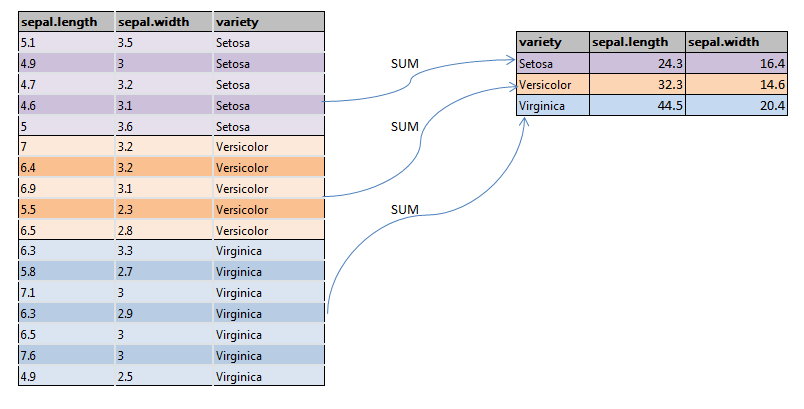
\includegraphics[width=1\linewidth,height=1\textheight]{imagem/group_by} 

}

\caption{ }\label{fig:group_by, figures-side}
\end{figure}

\hypertarget{funuxe7uxf5es-group_by-e-summarize-2}{%
\section{Funções group\_by e
summarize}\label{funuxe7uxf5es-group_by-e-summarize-2}}

\begin{Shaded}
\begin{Highlighting}[]
\NormalTok{basePaises }\OperatorTok
\StringTok{  }\KeywordTok{group_by}\NormalTok{(continent,year) }\OperatorTok
\StringTok{  }\KeywordTok{summarize}\NormalTok{(}\DataTypeTok{meanLE=}\KeywordTok{mean}\NormalTok{(lifeExp),}\DataTypeTok{meanPop=}\KeywordTok{mean}\NormalTok{(pop),}\DataTypeTok{meanGpc=}\KeywordTok{mean}\NormalTok{(gdpPercap))}
\end{Highlighting}
\end{Shaded}

\begin{verbatim}
## `summarise()` has grouped output by 'continent'. You can override using the `.groups` argument.
\end{verbatim}

\begin{verbatim}
## # A tibble: 60 x 5
## # Groups:   continent [5]
##    continent  year meanLE   meanPop meanGpc
##    <fct>     <int>  <dbl>     <dbl>   <dbl>
##  1 Africa     1952   39.1  4570010.   1253.
##  2 Africa     1957   41.3  5093033.   1385.
##  3 Africa     1962   43.3  5702247.   1598.
##  4 Africa     1967   45.3  6447875.   2050.
##  5 Africa     1972   47.5  7305376.   2340.
##  6 Africa     1977   49.6  8328097.   2586.
##  7 Africa     1982   51.6  9602857.   2482.
##  8 Africa     1987   53.3 11054502.   2283.
##  9 Africa     1992   53.6 12674645.   2282.
## 10 Africa     1997   53.6 14304480.   2379.
## # ... with 50 more rows
\end{verbatim}

\hypertarget{funuxe7uxf5es-top_n-e-arrange}{%
\section{Funções top\_n e arrange}\label{funuxe7uxf5es-top_n-e-arrange}}

A função top\_n serve para selecionar os n maiores valores que desejar

\begin{Shaded}
\begin{Highlighting}[]
\NormalTok{basePaises }\OperatorTok\StringTok{ }
\StringTok{  }\KeywordTok{filter}\NormalTok{(year }\OperatorTok{==}\StringTok{ }\DecValTok{2007}\NormalTok{) }\OperatorTok\StringTok{ }
\StringTok{  }\KeywordTok{top_n}\NormalTok{(}\DecValTok{5}\NormalTok{,pop) }\OperatorTok\StringTok{ }
\StringTok{  }\KeywordTok{arrange}\NormalTok{(}\KeywordTok{desc}\NormalTok{(pop))}
\end{Highlighting}
\end{Shaded}

\begin{verbatim}
## # A tibble: 5 x 7
##   country       continent  year lifeExp        pop gdpPercap     GDP
##   <fct>         <fct>     <int>   <dbl>      <int>     <dbl>   <dbl>
## 1 China         Asia       2007    73.0 1318683096     4959. 6.54e12
## 2 India         Asia       2007    64.7 1110396331     2452. 2.72e12
## 3 United States Americas   2007    78.2  301139947    42952. 1.29e13
## 4 Indonesia     Asia       2007    70.6  223547000     3541. 7.92e11
## 5 Brazil        Americas   2007    72.4  190010647     9066. 1.72e12
\end{verbatim}

\hypertarget{base-ice}{%
\section{Base ICE}\label{base-ice}}

\begin{figure}

{\centering 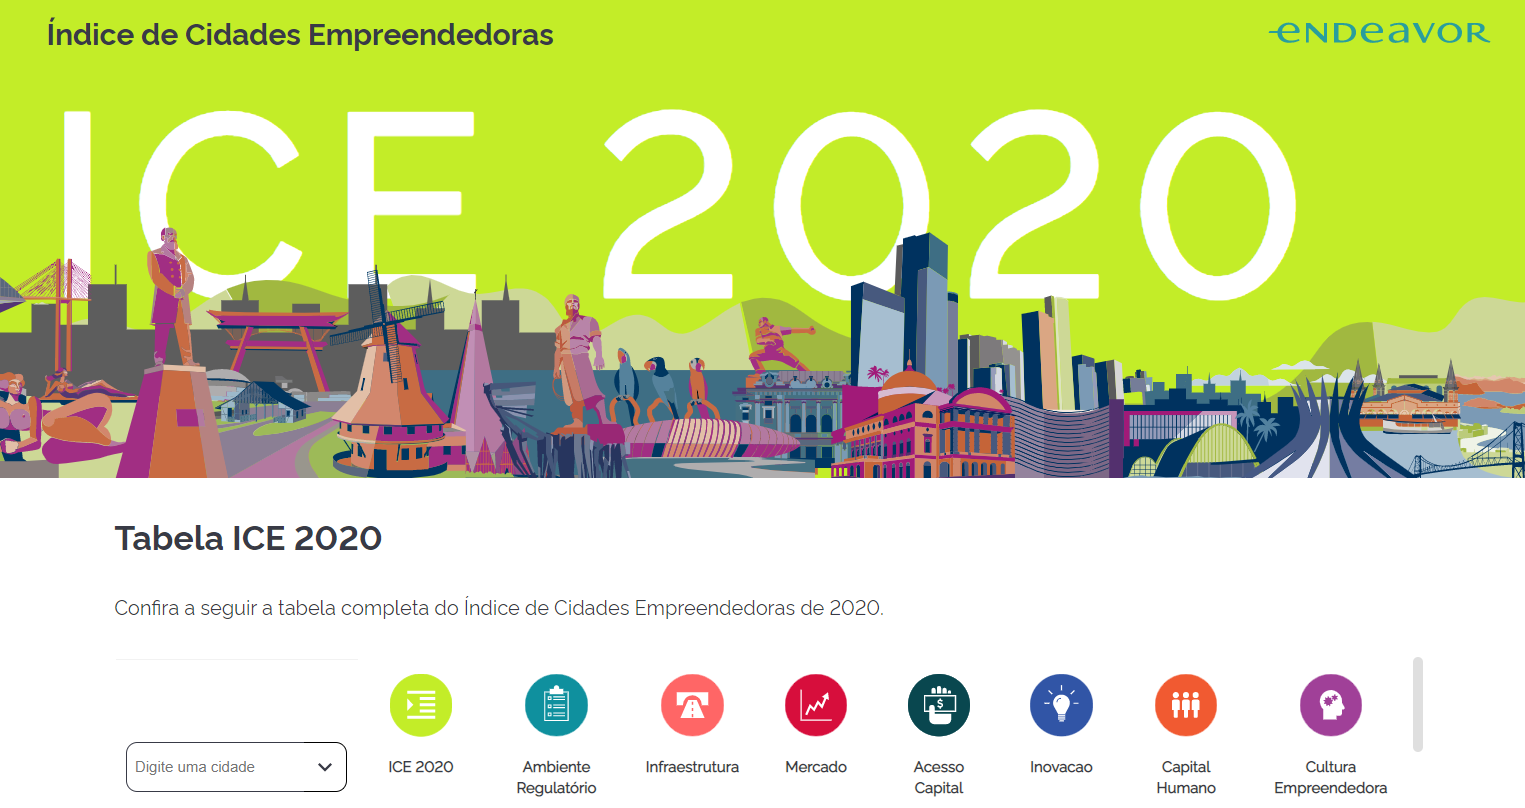
\includegraphics[width=1\linewidth,height=1\textheight]{imagem/ice} 

}

\caption{ }\label{fig:ice, figures-side}
\end{figure}

Fonte: \href{https://ice.enap.gov.br/}{Índice de Cidades empreendedoras}

\hypertarget{joins}{%
\section{Joins}\label{joins}}

\begin{Shaded}
\begin{Highlighting}[]
\NormalTok{munic <-}\StringTok{ }\KeywordTok{read.csv}\NormalTok{(}\StringTok{"https://raw.githubusercontent.com/danielppagotto/R_empreendedorismo1/main/arquivos%20de%20bases/politicas_empreendedorismo.csv"}\NormalTok{,}\DataTypeTok{sep =} \StringTok{";"}\NormalTok{, }\DataTypeTok{encoding =} \StringTok{"UTF-8"}\NormalTok{)}
\end{Highlighting}
\end{Shaded}

\hypertarget{introduzindo-funuxe7uxf5es-para-visualizauxe7uxe3o-de-dados}{%
\section{Introduzindo funções para visualização de
dados}\label{introduzindo-funuxe7uxf5es-para-visualizauxe7uxe3o-de-dados}}

\hypertarget{dica-de-leitura}{%
\section{Dica de leitura}\label{dica-de-leitura}}

\begin{figure}

{\centering 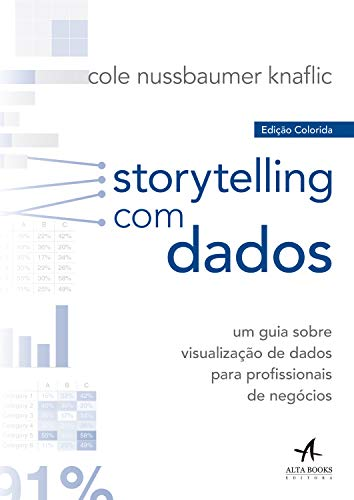
\includegraphics[width=0.4\linewidth,height=0.3\textheight]{imagem/storytelling} 

}

\caption{ }\label{fig:livro, figures-side}
\end{figure}

\hypertarget{preparando-nosso-ambiente}{%
\section{Preparando nosso ambiente}\label{preparando-nosso-ambiente}}

Antes de começar, vamos chamar alguns pacotes e preparar uma base que
usaremos! Caso não tenha algum dos pacotes abaixo ainda, terá que baixar
usando o comando \textbf{install.packages(``nome do pacote'')}.

\begin{Shaded}
\begin{Highlighting}[]
\KeywordTok{library}\NormalTok{(ggplot2)}
\KeywordTok{library}\NormalTok{(dplyr)}
\KeywordTok{library}\NormalTok{(gapminder)}

\NormalTok{base <-}\StringTok{ }\NormalTok{gapminder }\OperatorTok\StringTok{ }
\StringTok{  }\KeywordTok{filter}\NormalTok{(year }\OperatorTok{==}\StringTok{ }\DecValTok{2007}\NormalTok{) }

\KeywordTok{glimpse}\NormalTok{(base)}
\end{Highlighting}
\end{Shaded}

\begin{verbatim}
## Rows: 142
## Columns: 6
## $ country   <fct> "Afghanistan", "Albania", "Algeria", "Angola", "Argentina", ~
## $ continent <fct> Asia, Europe, Africa, Africa, Americas, Oceania, Europe, Asi~
## $ year      <int> 2007, 2007, 2007, 2007, 2007, 2007, 2007, 2007, 2007, 2007, ~
## $ lifeExp   <dbl> 43.828, 76.423, 72.301, 42.731, 75.320, 81.235, 79.829, 75.6~
## $ pop       <int> 31889923, 3600523, 33333216, 12420476, 40301927, 20434176, 8~
## $ gdpPercap <dbl> 974.5803, 5937.0295, 6223.3675, 4797.2313, 12779.3796, 34435~
\end{verbatim}

\hypertarget{extra---skimr}{%
\section{Extra - skimr}\label{extra---skimr}}

\begin{Shaded}
\begin{Highlighting}[]
\KeywordTok{library}\NormalTok{(skimr)}
\end{Highlighting}
\end{Shaded}

\begin{verbatim}
## Warning: package 'skimr' was built under R version 4.0.5
\end{verbatim}

\begin{Shaded}
\begin{Highlighting}[]
\NormalTok{skimr}\OperatorTok{::}\KeywordTok{skim}\NormalTok{(base)}
\end{Highlighting}
\end{Shaded}

\begin{longtable}[]{@{}ll@{}}
\caption{Data summary}\tabularnewline
\toprule
\endhead
Name & base\tabularnewline
Number of rows & 142\tabularnewline
Number of columns & 6\tabularnewline
\_\_\_\_\_\_\_\_\_\_\_\_\_\_\_\_\_\_\_\_\_\_\_ &\tabularnewline
Column type frequency: &\tabularnewline
factor & 2\tabularnewline
numeric & 4\tabularnewline
\_\_\_\_\_\_\_\_\_\_\_\_\_\_\_\_\_\_\_\_\_\_\_\_ &\tabularnewline
Group variables & None\tabularnewline
\bottomrule
\end{longtable}

\textbf{Variable type: factor}

\begin{longtable}[]{@{}lrrlrl@{}}
\toprule
skim\_variable & n\_missing & complete\_rate & ordered & n\_unique &
top\_counts\tabularnewline
\midrule
\endhead
country & 0 & 1 & FALSE & 142 & Afg: 1, Alb: 1, Alg: 1, Ang:
1\tabularnewline
continent & 0 & 1 & FALSE & 5 & Afr: 52, Asi: 33, Eur: 30, Ame:
25\tabularnewline
\bottomrule
\end{longtable}

\textbf{Variable type: numeric}

\begin{longtable}[]{@{}lrrrrrrrrrl@{}}
\toprule
\begin{minipage}[b]{0.06\columnwidth}\raggedright
skim\_variable\strut
\end{minipage} & \begin{minipage}[b]{0.04\columnwidth}\raggedleft
n\_missing\strut
\end{minipage} & \begin{minipage}[b]{0.06\columnwidth}\raggedleft
complete\_rate\strut
\end{minipage} & \begin{minipage}[b]{0.05\columnwidth}\raggedleft
mean\strut
\end{minipage} & \begin{minipage}[b]{0.06\columnwidth}\raggedleft
sd\strut
\end{minipage} & \begin{minipage}[b]{0.04\columnwidth}\raggedleft
p0\strut
\end{minipage} & \begin{minipage}[b]{0.05\columnwidth}\raggedleft
p25\strut
\end{minipage} & \begin{minipage}[b]{0.05\columnwidth}\raggedleft
p50\strut
\end{minipage} & \begin{minipage}[b]{0.05\columnwidth}\raggedleft
p75\strut
\end{minipage} & \begin{minipage}[b]{0.06\columnwidth}\raggedleft
p100\strut
\end{minipage} & \begin{minipage}[b]{0.18\columnwidth}\raggedright
hist\strut
\end{minipage}\tabularnewline
\midrule
\endhead
\begin{minipage}[t]{0.06\columnwidth}\raggedright
year\strut
\end{minipage} & \begin{minipage}[t]{0.04\columnwidth}\raggedleft
0\strut
\end{minipage} & \begin{minipage}[t]{0.06\columnwidth}\raggedleft
1\strut
\end{minipage} & \begin{minipage}[t]{0.05\columnwidth}\raggedleft
2007.00\strut
\end{minipage} & \begin{minipage}[t]{0.06\columnwidth}\raggedleft
0.00\strut
\end{minipage} & \begin{minipage}[t]{0.04\columnwidth}\raggedleft
2007.00\strut
\end{minipage} & \begin{minipage}[t]{0.05\columnwidth}\raggedleft
2007.00\strut
\end{minipage} & \begin{minipage}[t]{0.05\columnwidth}\raggedleft
2007.00\strut
\end{minipage} & \begin{minipage}[t]{0.05\columnwidth}\raggedleft
2007.00\strut
\end{minipage} & \begin{minipage}[t]{0.06\columnwidth}\raggedleft
2.007000e+03\strut
\end{minipage} & \begin{minipage}[t]{0.18\columnwidth}\raggedright
▁▁▇▁▁\strut
\end{minipage}\tabularnewline
\begin{minipage}[t]{0.06\columnwidth}\raggedright
lifeExp\strut
\end{minipage} & \begin{minipage}[t]{0.04\columnwidth}\raggedleft
0\strut
\end{minipage} & \begin{minipage}[t]{0.06\columnwidth}\raggedleft
1\strut
\end{minipage} & \begin{minipage}[t]{0.05\columnwidth}\raggedleft
67.01\strut
\end{minipage} & \begin{minipage}[t]{0.06\columnwidth}\raggedleft
12.07\strut
\end{minipage} & \begin{minipage}[t]{0.04\columnwidth}\raggedleft
39.61\strut
\end{minipage} & \begin{minipage}[t]{0.05\columnwidth}\raggedleft
57.16\strut
\end{minipage} & \begin{minipage}[t]{0.05\columnwidth}\raggedleft
71.94\strut
\end{minipage} & \begin{minipage}[t]{0.05\columnwidth}\raggedleft
76.41\strut
\end{minipage} & \begin{minipage}[t]{0.06\columnwidth}\raggedleft
8.260000e+01\strut
\end{minipage} & \begin{minipage}[t]{0.18\columnwidth}\raggedright
▂▃▃▆▇\strut
\end{minipage}\tabularnewline
\begin{minipage}[t]{0.06\columnwidth}\raggedright
pop\strut
\end{minipage} & \begin{minipage}[t]{0.04\columnwidth}\raggedleft
0\strut
\end{minipage} & \begin{minipage}[t]{0.06\columnwidth}\raggedleft
1\strut
\end{minipage} & \begin{minipage}[t]{0.05\columnwidth}\raggedleft
44021219.57\strut
\end{minipage} & \begin{minipage}[t]{0.06\columnwidth}\raggedleft
147621397.90\strut
\end{minipage} & \begin{minipage}[t]{0.04\columnwidth}\raggedleft
199579.00\strut
\end{minipage} & \begin{minipage}[t]{0.05\columnwidth}\raggedleft
4508033.50\strut
\end{minipage} & \begin{minipage}[t]{0.05\columnwidth}\raggedleft
10517531.00\strut
\end{minipage} & \begin{minipage}[t]{0.05\columnwidth}\raggedleft
31210041.75\strut
\end{minipage} & \begin{minipage}[t]{0.06\columnwidth}\raggedleft
1.318683e+09\strut
\end{minipage} & \begin{minipage}[t]{0.18\columnwidth}\raggedright
▇▁▁▁▁\strut
\end{minipage}\tabularnewline
\begin{minipage}[t]{0.06\columnwidth}\raggedright
gdpPercap\strut
\end{minipage} & \begin{minipage}[t]{0.04\columnwidth}\raggedleft
0\strut
\end{minipage} & \begin{minipage}[t]{0.06\columnwidth}\raggedleft
1\strut
\end{minipage} & \begin{minipage}[t]{0.05\columnwidth}\raggedleft
11680.07\strut
\end{minipage} & \begin{minipage}[t]{0.06\columnwidth}\raggedleft
12859.94\strut
\end{minipage} & \begin{minipage}[t]{0.04\columnwidth}\raggedleft
277.55\strut
\end{minipage} & \begin{minipage}[t]{0.05\columnwidth}\raggedleft
1624.84\strut
\end{minipage} & \begin{minipage}[t]{0.05\columnwidth}\raggedleft
6124.37\strut
\end{minipage} & \begin{minipage}[t]{0.05\columnwidth}\raggedleft
18008.84\strut
\end{minipage} & \begin{minipage}[t]{0.06\columnwidth}\raggedleft
4.935719e+04\strut
\end{minipage} & \begin{minipage}[t]{0.18\columnwidth}\raggedright
▇▂▁▂▁\strut
\end{minipage}\tabularnewline
\bottomrule
\end{longtable}

\hypertarget{curiosidade}{%
\section{Curiosidade! ;)}\label{curiosidade}}

\textbf{FYI:} Gapminder é uma organização sem fins lucrativos que
promove o desenvolvimento e atingimento dos ODS ao difundir a
compreensão de informações de ordem social, econômica, ambiental a nível
local, nacional e global.

\begin{center}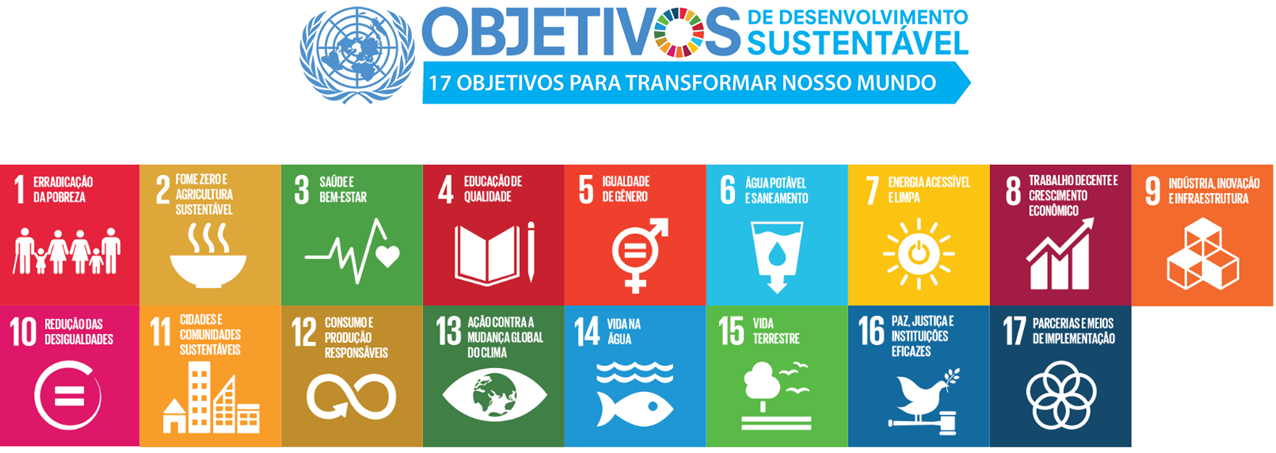
\includegraphics[width=17.72in]{imagem/ODS} \end{center}

\hypertarget{ggplot2---a-base-de-tudo}{%
\section{GGPlot2 - a base de tudo}\label{ggplot2---a-base-de-tudo}}

O R por si só possui funções para gerar gráficos, porém o ggplot2 é um
pacote que fornece um conjunto bem extenso de possibilidades

\begin{Shaded}
\begin{Highlighting}[]
\KeywordTok{hist}\NormalTok{(base}\OperatorTok{$}\NormalTok{lifeExp)}
\end{Highlighting}
\end{Shaded}

\begin{center}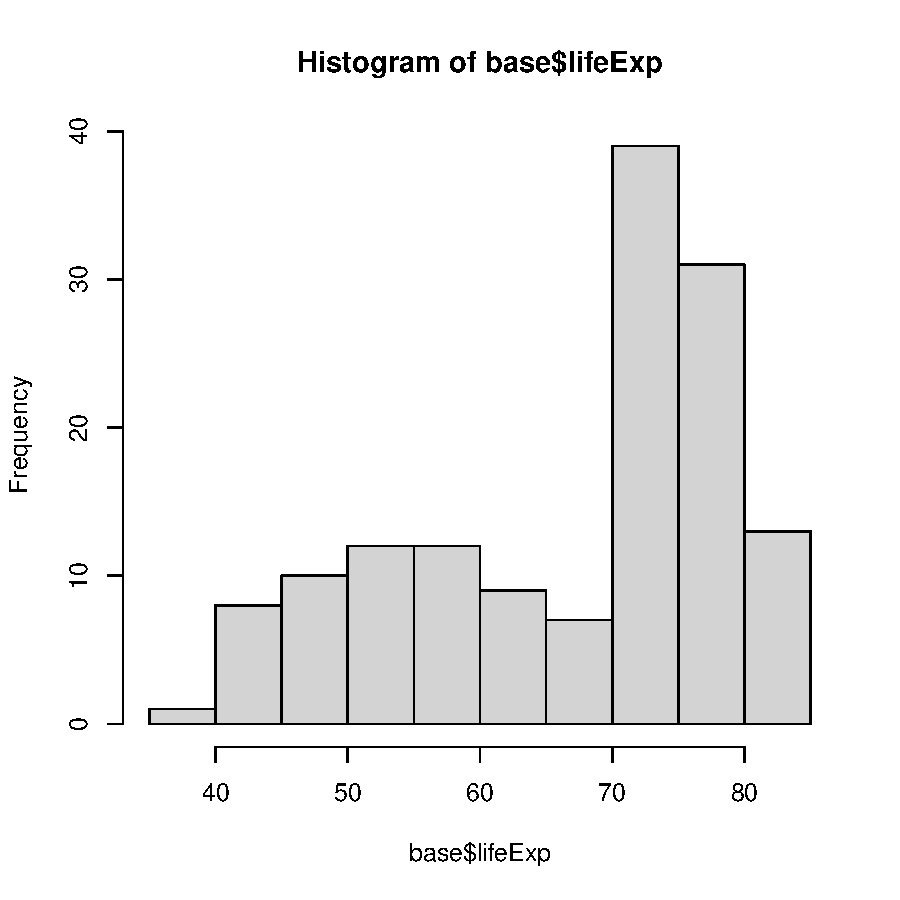
\includegraphics{arquivo_pdf_files/figure-latex/histograma1-1} \end{center}

\hypertarget{ggplot2---a-base-de-tudo-1}{%
\section{GGPlot2 - a base de tudo}\label{ggplot2---a-base-de-tudo-1}}

Vamos criar um histograma sobre a variável expectativa de vida.

\begin{Shaded}
\begin{Highlighting}[]
\KeywordTok{ggplot}\NormalTok{(base, }\KeywordTok{aes}\NormalTok{(}\DataTypeTok{x =}\NormalTok{ lifeExp)) }\OperatorTok{+}\StringTok{ }\KeywordTok{geom_histogram}\NormalTok{()}
\end{Highlighting}
\end{Shaded}

\begin{center}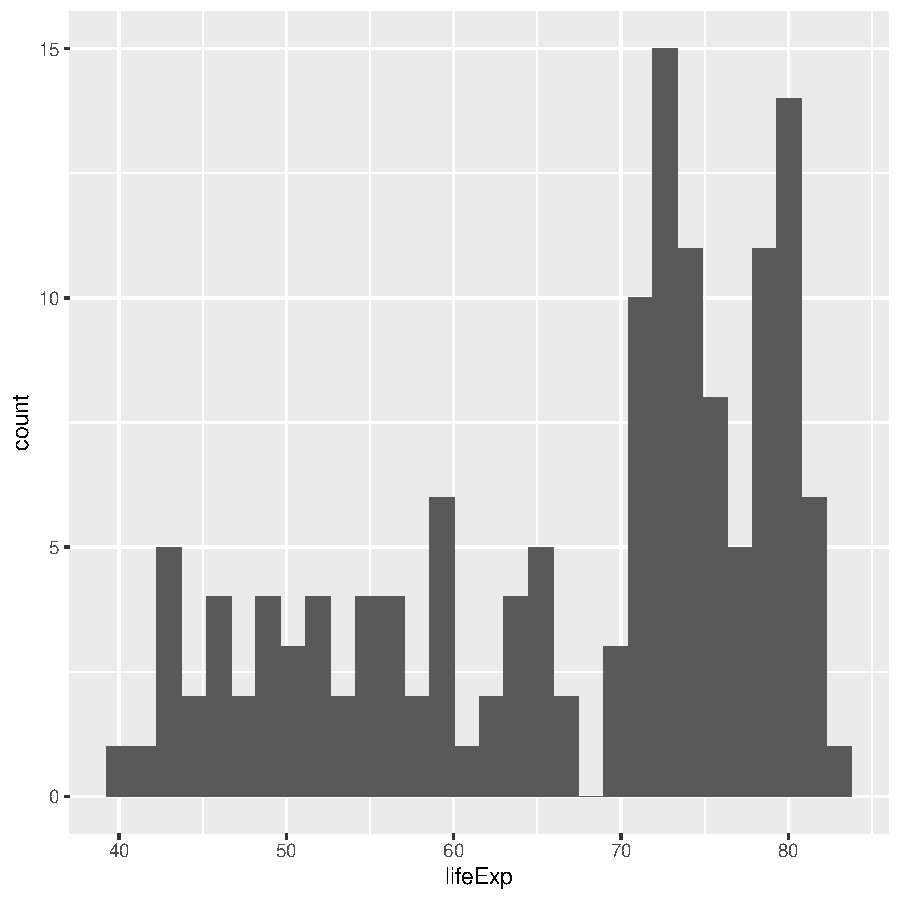
\includegraphics{arquivo_pdf_files/figure-latex/histograma2-1} \end{center}

\hypertarget{ggplot2---densidade}{%
\section{GGPlot2 - Densidade}\label{ggplot2---densidade}}

Vamos criar um gráfico de densidade sobre a variável expectativa de
vida. Veja outra forma de usar a função ggplot.

\begin{Shaded}
\begin{Highlighting}[]
\NormalTok{base }\OperatorTok\StringTok{ }
\StringTok{  }\KeywordTok{ggplot}\NormalTok{(}\KeywordTok{aes}\NormalTok{(}\DataTypeTok{x =}\NormalTok{ lifeExp)) }\OperatorTok{+}\StringTok{ }\KeywordTok{geom_density}\NormalTok{()}
\end{Highlighting}
\end{Shaded}

\begin{center}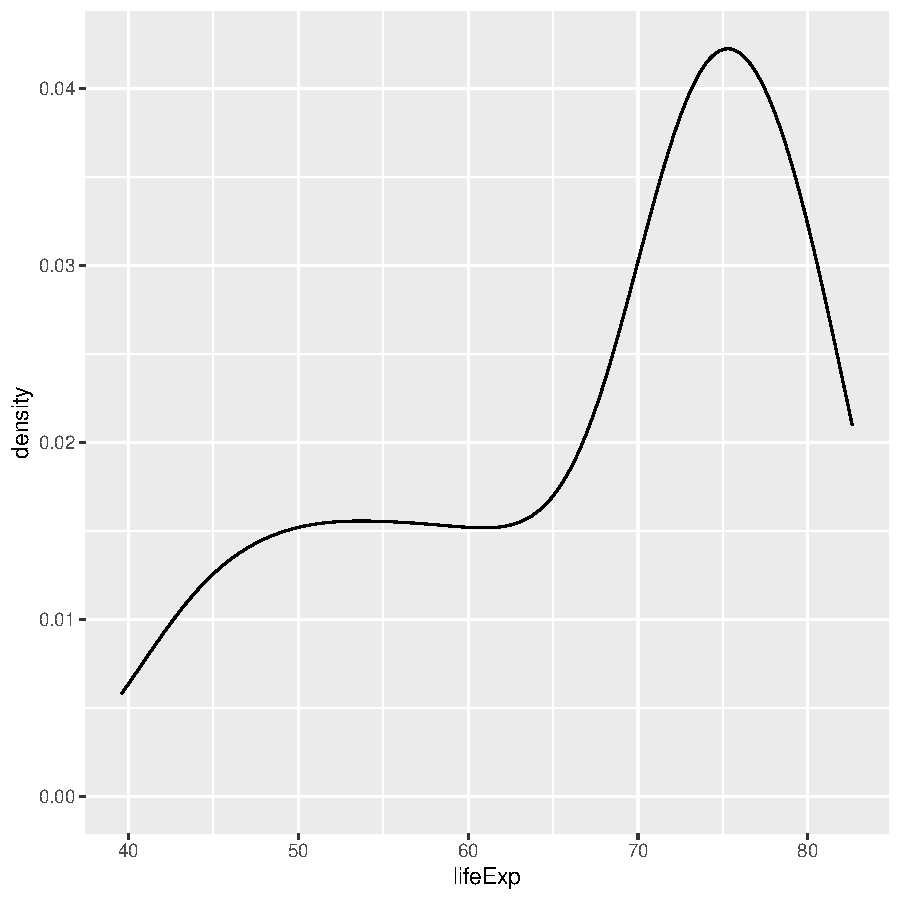
\includegraphics{arquivo_pdf_files/figure-latex/densidade-1} \end{center}

\hypertarget{ggplot2---boxplot}{%
\section{GGPlot2 - Boxplot}\label{ggplot2---boxplot}}

Vamos criar um boxplot sobre a variável expectativa de vida.

\begin{Shaded}
\begin{Highlighting}[]
\NormalTok{base }\OperatorTok\StringTok{ }
\StringTok{  }\KeywordTok{ggplot}\NormalTok{(}\KeywordTok{aes}\NormalTok{(}\DataTypeTok{y =}\NormalTok{ lifeExp)) }\OperatorTok{+}\StringTok{ }\KeywordTok{geom_boxplot}\NormalTok{()}
\end{Highlighting}
\end{Shaded}

\begin{center}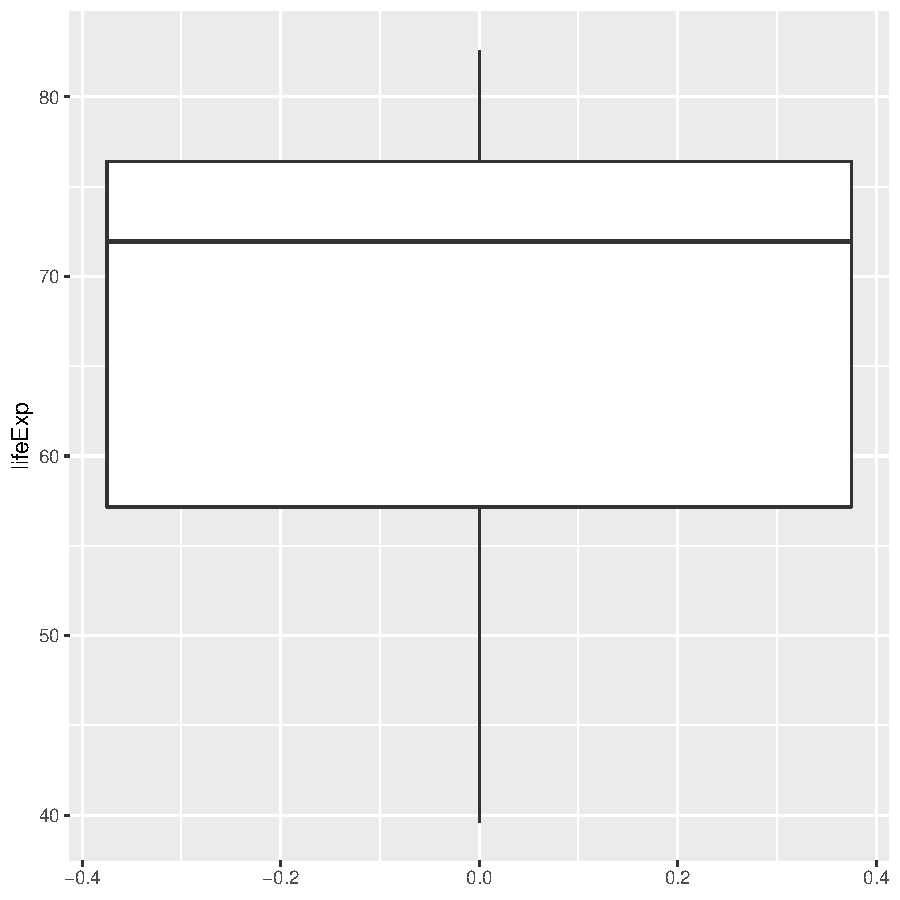
\includegraphics{arquivo_pdf_files/figure-latex/boxplot1-1} \end{center}

\hypertarget{ggplot2---boxplot-2}{%
\section{GGPlot2 - Boxplot 2}\label{ggplot2---boxplot-2}}

Vamos criar um boxplot sobre a variável expectativa de vida.

\begin{Shaded}
\begin{Highlighting}[]
\NormalTok{base }\OperatorTok\StringTok{ }
\StringTok{  }\KeywordTok{ggplot}\NormalTok{(}\KeywordTok{aes}\NormalTok{(}\DataTypeTok{x =}\NormalTok{ continent, }\DataTypeTok{y =}\NormalTok{ lifeExp)) }\OperatorTok{+}\StringTok{ }\KeywordTok{geom_boxplot}\NormalTok{()}
\end{Highlighting}
\end{Shaded}

\begin{center}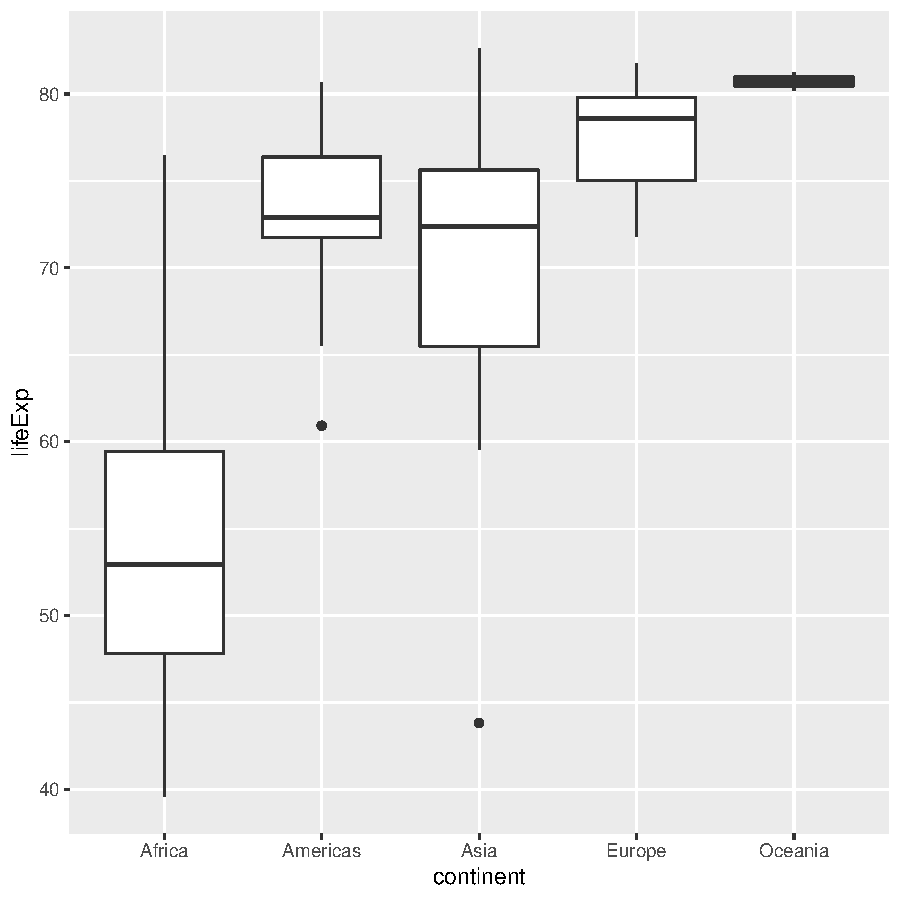
\includegraphics{arquivo_pdf_files/figure-latex/boxplot2-1} \end{center}

\hypertarget{ggplot2---gruxe1fico-de-colunas}{%
\section{GGPlot2 - Gráfico de
colunas}\label{ggplot2---gruxe1fico-de-colunas}}

Vamos criar um gráfico de barras da variável expectativa de vida. Nesse
caso, vamos pegar os 10 países da Ásia com maior taxa de expectativa de
vida.

\begin{Shaded}
\begin{Highlighting}[]
\NormalTok{base }\OperatorTok\StringTok{ }
\StringTok{  }\KeywordTok{filter}\NormalTok{(continent }\OperatorTok{==}\StringTok{ "Asia"}\NormalTok{) }\OperatorTok\StringTok{ }
\StringTok{  }\KeywordTok{top_n}\NormalTok{(}\DataTypeTok{n =} \DecValTok{10}\NormalTok{, }\DataTypeTok{wt =}\NormalTok{ lifeExp) }\OperatorTok\StringTok{ }
\StringTok{  }\KeywordTok{ggplot}\NormalTok{(}\KeywordTok{aes}\NormalTok{(}\DataTypeTok{x =}\NormalTok{ country, }\DataTypeTok{y =}\NormalTok{ lifeExp)) }\OperatorTok{+}\StringTok{ }\KeywordTok{geom_col}\NormalTok{() }
\end{Highlighting}
\end{Shaded}

\begin{center}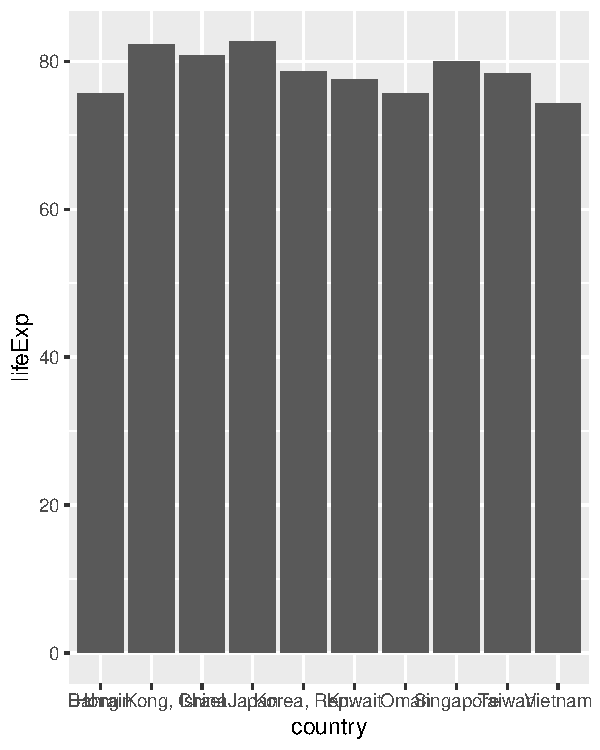
\includegraphics{arquivo_pdf_files/figure-latex/barras-1} \end{center}

\hypertarget{ggplot2---coord_flip}{%
\section{GGPlot2 - Coord\_flip}\label{ggplot2---coord_flip}}

Veja como melhorar a visualização com um simples argumento

\begin{Shaded}
\begin{Highlighting}[]
\NormalTok{base }\OperatorTok\StringTok{ }
\StringTok{  }\KeywordTok{filter}\NormalTok{(continent }\OperatorTok{==}\StringTok{ "Asia"}\NormalTok{) }\OperatorTok\StringTok{ }
\StringTok{  }\KeywordTok{top_n}\NormalTok{(}\DataTypeTok{n =} \DecValTok{10}\NormalTok{, }\DataTypeTok{wt =}\NormalTok{ lifeExp) }\OperatorTok\StringTok{ }
\StringTok{  }\KeywordTok{ggplot}\NormalTok{(}\KeywordTok{aes}\NormalTok{(}\DataTypeTok{x =}\NormalTok{ country, }\DataTypeTok{y =}\NormalTok{ lifeExp)) }\OperatorTok{+}\StringTok{ }\KeywordTok{geom_col}\NormalTok{() }\OperatorTok{+}\StringTok{ }\KeywordTok{coord_flip}\NormalTok{()}
\end{Highlighting}
\end{Shaded}

\begin{center}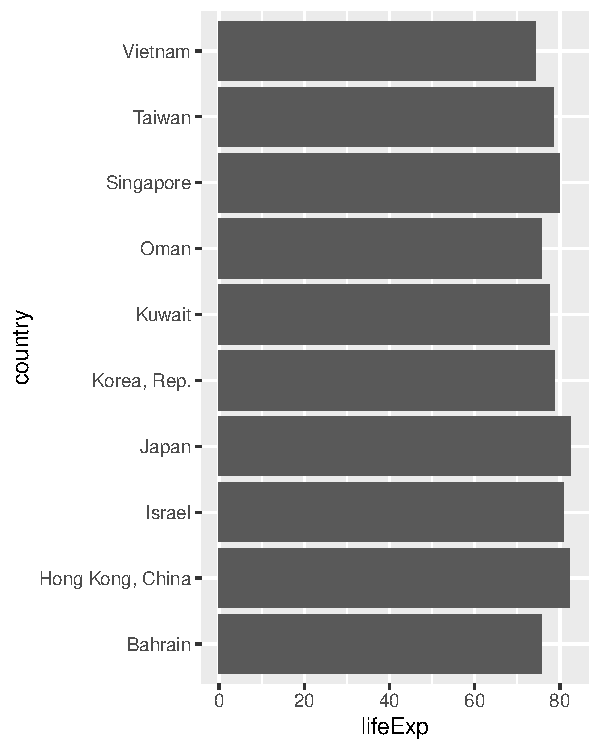
\includegraphics{arquivo_pdf_files/figure-latex/barras2-1} \end{center}

\#Mas, Daniel, consigo deixar em ordem? Sim, para isso, vamos usar uma
função do pacote forcats.

\begin{Shaded}
\begin{Highlighting}[]
\KeywordTok{library}\NormalTok{(forcats)}
\NormalTok{base }\OperatorTok\StringTok{ }
\StringTok{  }\KeywordTok{filter}\NormalTok{(continent }\OperatorTok{==}\StringTok{ "Asia"}\NormalTok{) }\OperatorTok\StringTok{ }
\StringTok{  }\KeywordTok{top_n}\NormalTok{(}\DataTypeTok{n =} \DecValTok{10}\NormalTok{, }\DataTypeTok{wt =}\NormalTok{ lifeExp) }\OperatorTok\StringTok{ }
\StringTok{  }\KeywordTok{ggplot}\NormalTok{(}\KeywordTok{aes}\NormalTok{(}\DataTypeTok{x =} \KeywordTok{fct_reorder}\NormalTok{(country,lifeExp), }\DataTypeTok{y =}\NormalTok{ lifeExp)) }\OperatorTok{+}\StringTok{ }\KeywordTok{geom_col}\NormalTok{() }\OperatorTok{+}\StringTok{ }\KeywordTok{coord_flip}\NormalTok{()}
\end{Highlighting}
\end{Shaded}

\begin{center}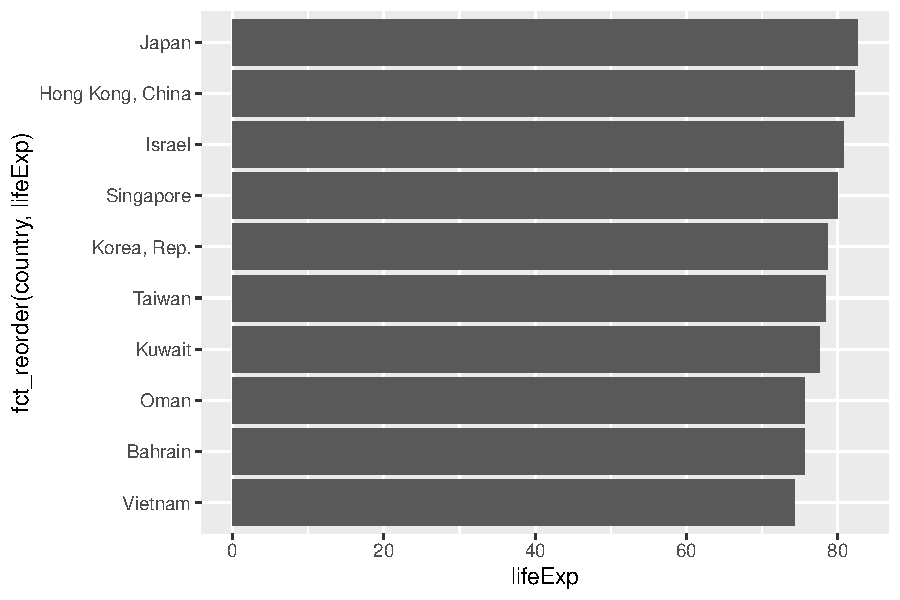
\includegraphics{arquivo_pdf_files/figure-latex/barras3-1} \end{center}

\hypertarget{ggplot2---labels}{%
\section{GGPlot2 - Labels}\label{ggplot2---labels}}

Adicionando labels

\begin{Shaded}
\begin{Highlighting}[]
\NormalTok{base }\OperatorTok\StringTok{ }
\StringTok{  }\KeywordTok{filter}\NormalTok{(continent }\OperatorTok{==}\StringTok{ "Asia"}\NormalTok{) }\OperatorTok\StringTok{ }
\StringTok{  }\KeywordTok{top_n}\NormalTok{(}\DataTypeTok{n =} \DecValTok{10}\NormalTok{, }\DataTypeTok{wt =}\NormalTok{ lifeExp) }\OperatorTok\StringTok{ }
\StringTok{  }\KeywordTok{ggplot}\NormalTok{(}\KeywordTok{aes}\NormalTok{(}\DataTypeTok{x =} \KeywordTok{fct_reorder}\NormalTok{(country,lifeExp), }\DataTypeTok{y =}\NormalTok{ lifeExp)) }\OperatorTok{+}\StringTok{ }\KeywordTok{geom_col}\NormalTok{() }\OperatorTok{+}\StringTok{ }
\StringTok{  }\KeywordTok{geom_label}\NormalTok{(}\KeywordTok{aes}\NormalTok{(}\DataTypeTok{label=}\KeywordTok{round}\NormalTok{(lifeExp))) }\OperatorTok{+}\StringTok{  }\KeywordTok{coord_flip}\NormalTok{()}
\end{Highlighting}
\end{Shaded}

\begin{center}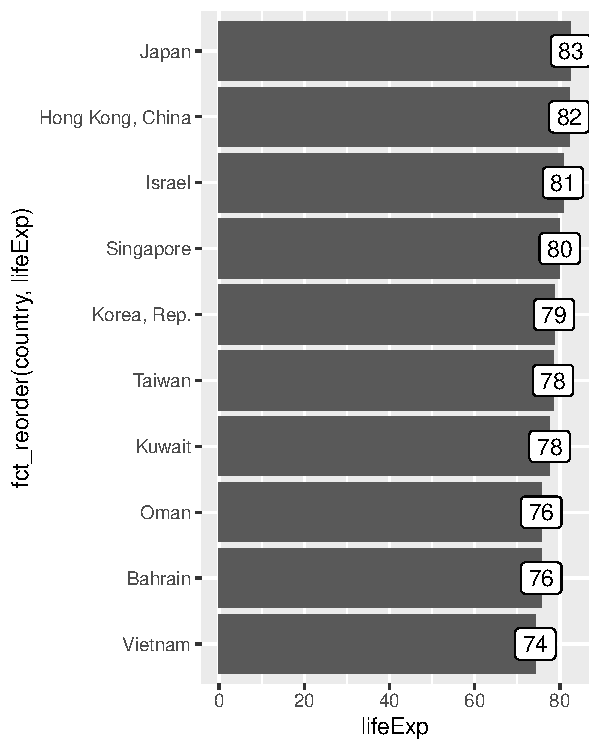
\includegraphics{arquivo_pdf_files/figure-latex/barras4-1} \end{center}

\hypertarget{ggplot2---linhas}{%
\section{GGPlot2 - Linhas}\label{ggplot2---linhas}}

Para fazer esse gráfico, vamos usar a base original, gapminder, e
filtrar apenas o Brasil.

\begin{Shaded}
\begin{Highlighting}[]
\NormalTok{gapminder }\OperatorTok\StringTok{ }
\StringTok{  }\KeywordTok{filter}\NormalTok{(country }\OperatorTok{==}\StringTok{ "Brazil"}\NormalTok{) }\OperatorTok\StringTok{ }
\StringTok{  }\KeywordTok{ggplot}\NormalTok{(}\KeywordTok{aes}\NormalTok{(}\DataTypeTok{x =}\NormalTok{ year, }\DataTypeTok{y =}\NormalTok{ lifeExp)) }\OperatorTok{+}\StringTok{ }\KeywordTok{geom_line}\NormalTok{() }
\end{Highlighting}
\end{Shaded}

\begin{center}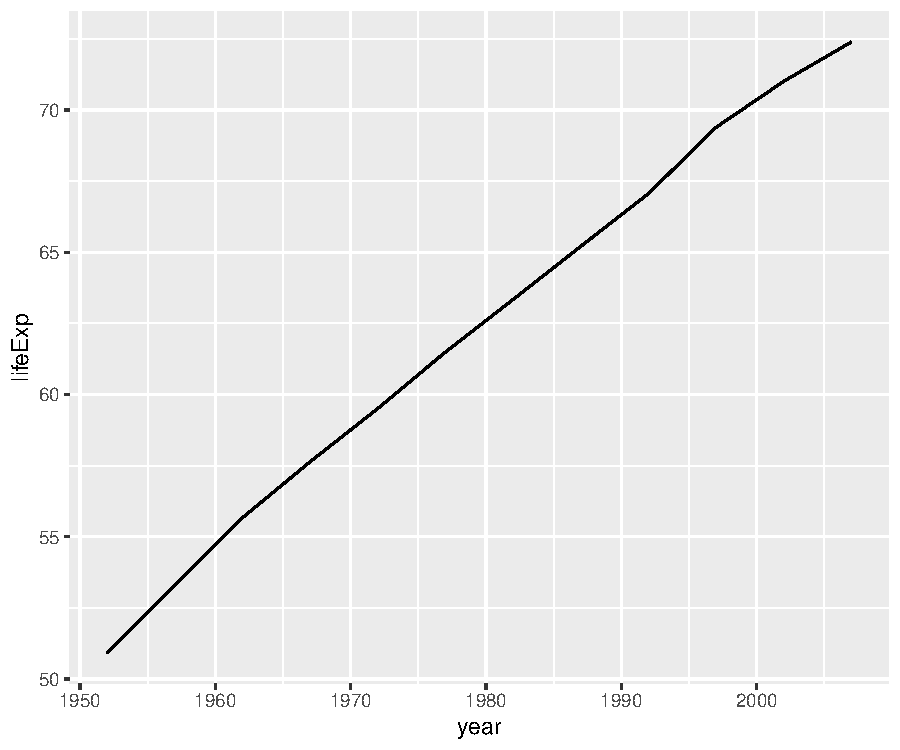
\includegraphics{arquivo_pdf_files/figure-latex/linhas-1} \end{center}

\hypertarget{ggplot2---argumento-col}{%
\section{GGPlot2 - Argumento col}\label{ggplot2---argumento-col}}

Veja que legal é o argumento col dentro do aes.

\begin{Shaded}
\begin{Highlighting}[]
\NormalTok{paises <-}\StringTok{ }\KeywordTok{c}\NormalTok{(}\StringTok{"Brazil"}\NormalTok{,}\StringTok{"Argentina"}\NormalTok{)}

\NormalTok{gapminder }\OperatorTok\StringTok{ }
\StringTok{  }\KeywordTok{filter}\NormalTok{(country }\OperatorTok\StringTok{ }\NormalTok{paises) }\OperatorTok\StringTok{ }
\StringTok{  }\KeywordTok{ggplot}\NormalTok{(}\KeywordTok{aes}\NormalTok{(}\DataTypeTok{x =}\NormalTok{ year, }\DataTypeTok{y =}\NormalTok{ lifeExp, }\DataTypeTok{col =}\NormalTok{ country)) }\OperatorTok{+}\StringTok{ }\KeywordTok{geom_line}\NormalTok{() }
\end{Highlighting}
\end{Shaded}

\begin{center}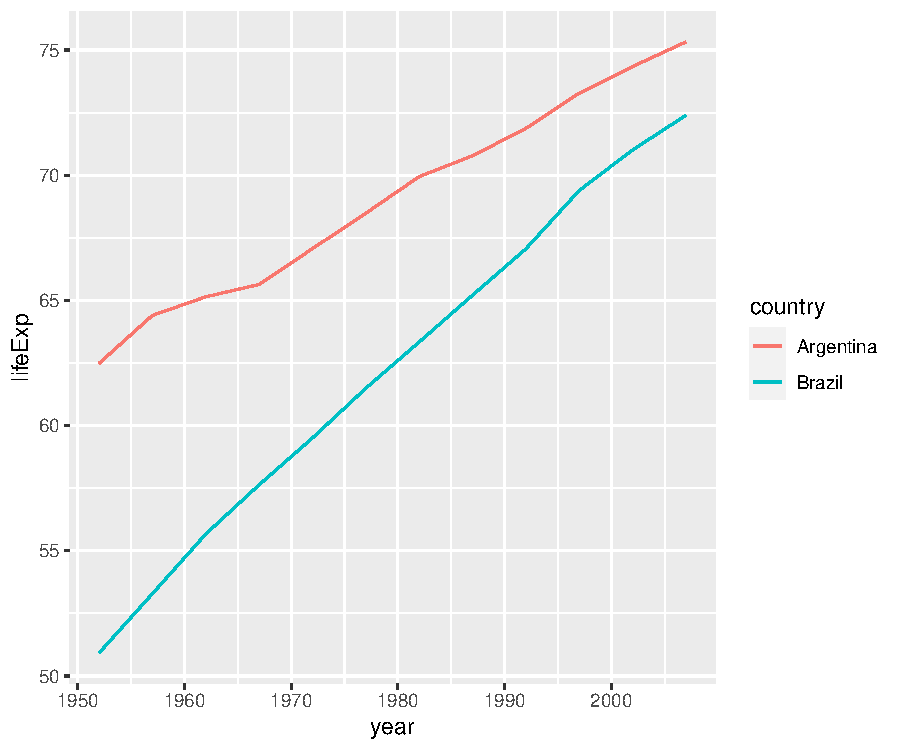
\includegraphics{arquivo_pdf_files/figure-latex/linhas2-1} \end{center}

\hypertarget{usando-argumento-fill}{%
\section{Usando argumento fill}\label{usando-argumento-fill}}

Vamos ver como funciona o argumento \texttt{fill}

\begin{Shaded}
\begin{Highlighting}[]
\NormalTok{base }\OperatorTok\StringTok{ }
\StringTok{  }\KeywordTok{top_n}\NormalTok{(}\DecValTok{10}\NormalTok{) }\OperatorTok\StringTok{ }
\StringTok{  }\KeywordTok{ggplot}\NormalTok{(}\KeywordTok{aes}\NormalTok{(}\DataTypeTok{x =} \KeywordTok{fct_reorder}\NormalTok{(country,gdpPercap), }\DataTypeTok{y=}\NormalTok{gdpPercap, }\DataTypeTok{fill =}\NormalTok{ continent)) }\OperatorTok{+}\StringTok{ }\KeywordTok{geom_col}\NormalTok{() }\OperatorTok{+}\StringTok{ }\KeywordTok{coord_flip}\NormalTok{()}
\end{Highlighting}
\end{Shaded}

\begin{center}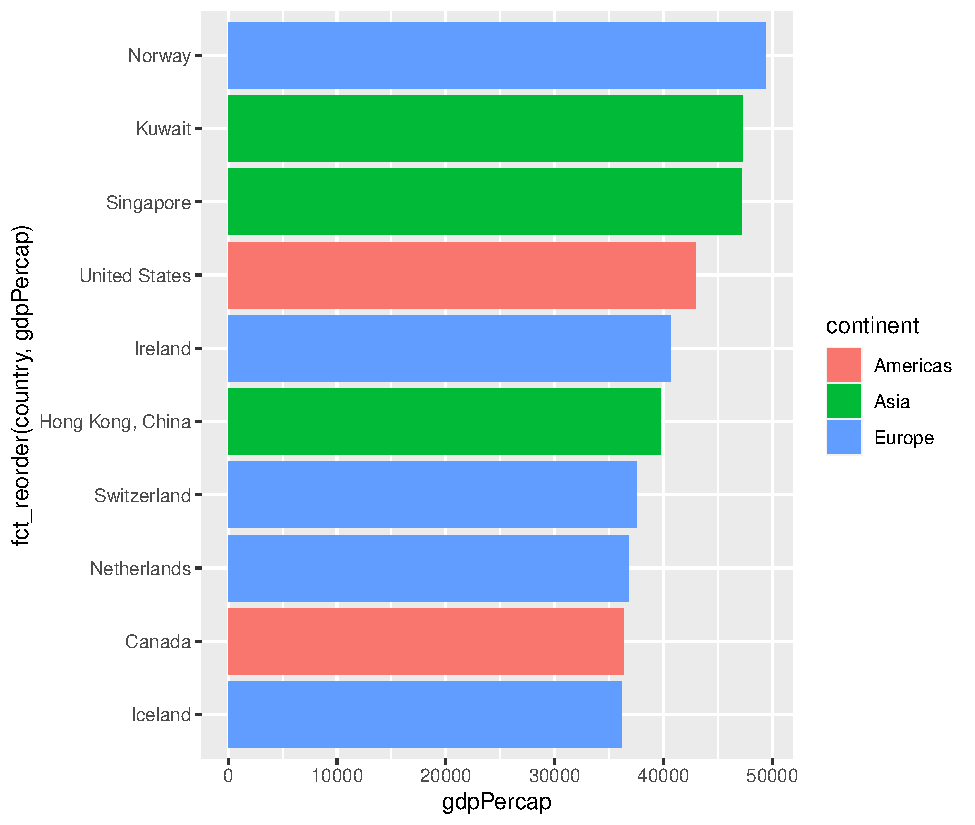
\includegraphics{arquivo_pdf_files/figure-latex/densidade_customizada2-1} \end{center}

\hypertarget{massa-daniel}{%
\section{Massa, Daniel!}\label{massa-daniel}}

Você falou que podíamos customizar muita coisa. E aí? Calma, jovem, veja
só\ldots{}

\begin{Shaded}
\begin{Highlighting}[]
\KeywordTok{ggplot}\NormalTok{(base,}\KeywordTok{aes}\NormalTok{(}\DataTypeTok{x=}\NormalTok{lifeExp)) }\OperatorTok{+}\StringTok{ }\KeywordTok{geom_density}\NormalTok{(}\DataTypeTok{fill=}\StringTok{"darkblue"}\NormalTok{) }\OperatorTok{+}
\StringTok{  }\KeywordTok{labs}\NormalTok{(}\DataTypeTok{title =} \StringTok{"Histograma da expectativa de vida"}\NormalTok{, }
       \DataTypeTok{x =} \StringTok{"Expectativa de vida"}\NormalTok{, }\DataTypeTok{y =} \StringTok{"Frequência") + theme_minimal()}
\end{Highlighting}
\end{Shaded}

\begin{center}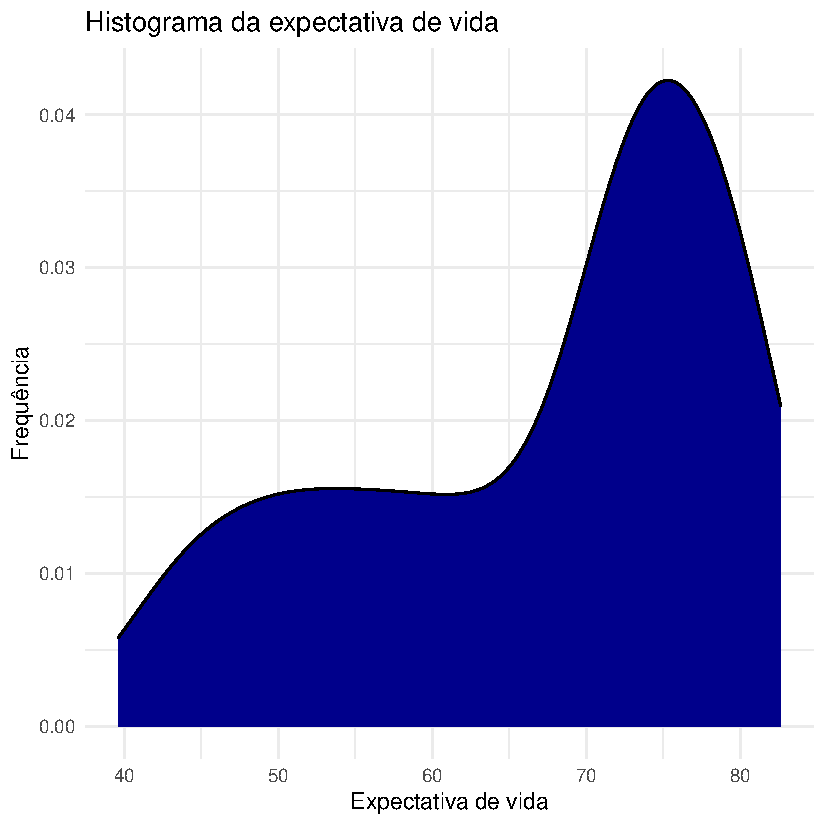
\includegraphics{arquivo_pdf_files/figure-latex/densidade customizada-1} \end{center}

\hypertarget{vamos-trabalhar-com-duas-variuxe1veis}{%
\section{Vamos trabalhar com duas
variáveis\ldots{}}\label{vamos-trabalhar-com-duas-variuxe1veis}}

Vamos relacionar duas variáveis: PIB per capita e expectativa de vida

\begin{Shaded}
\begin{Highlighting}[]
\KeywordTok{ggplot}\NormalTok{(base,}\KeywordTok{aes}\NormalTok{(}\DataTypeTok{x=}\KeywordTok{log}\NormalTok{(gdpPercap),}\DataTypeTok{y=}\NormalTok{lifeExp)) }\OperatorTok{+}\StringTok{ }\KeywordTok{geom_point}\NormalTok{() }\OperatorTok{+}
\StringTok{  }\KeywordTok{labs}\NormalTok{(}\DataTypeTok{x =} \StringTok{"PIB per capita (log)"}\NormalTok{, }\DataTypeTok{y =} \StringTok{"Expectativa de vida"}\NormalTok{) }\OperatorTok{+}\StringTok{ }\KeywordTok{theme_bw}\NormalTok{()}
\end{Highlighting}
\end{Shaded}

\begin{center}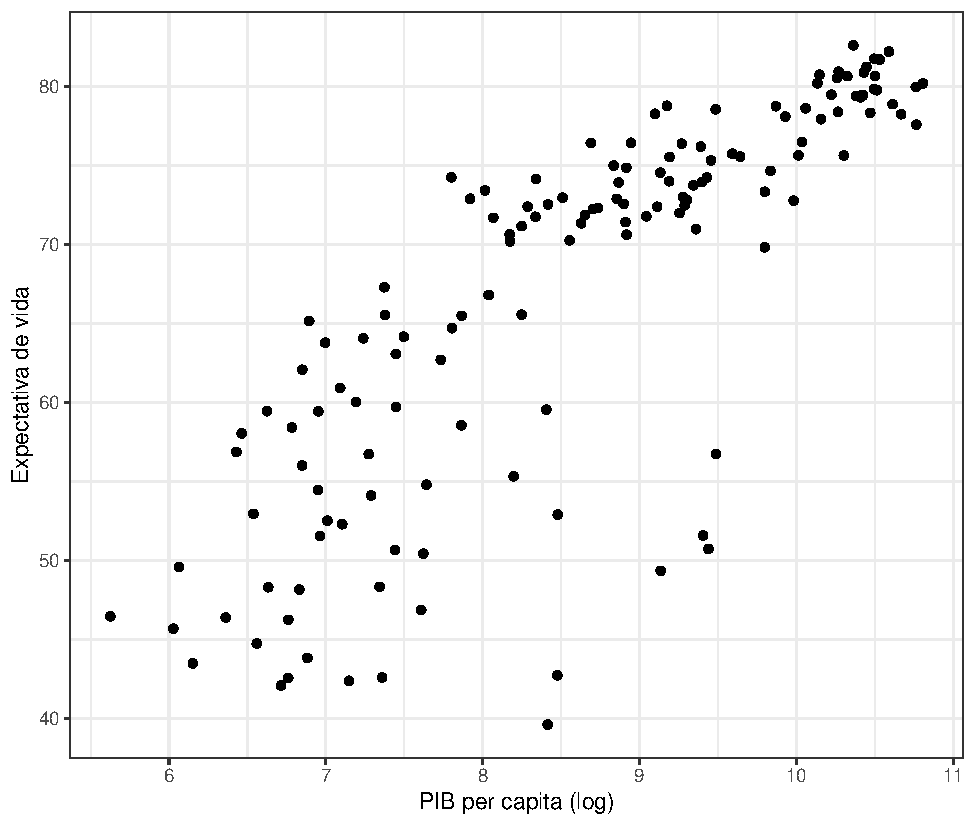
\includegraphics{arquivo_pdf_files/figure-latex/scatter-1} \end{center}

\hypertarget{mais-uma-camada}{%
\section{Mais uma camada\ldots{}}\label{mais-uma-camada}}

\begin{Shaded}
\begin{Highlighting}[]
\KeywordTok{ggplot}\NormalTok{(base,}\KeywordTok{aes}\NormalTok{(}\DataTypeTok{y=}\NormalTok{lifeExp, }\DataTypeTok{x=}\KeywordTok{log}\NormalTok{(gdpPercap))) }\OperatorTok{+}\StringTok{ }\KeywordTok{geom_point}\NormalTok{() }\OperatorTok{+}
\StringTok{  }\KeywordTok{geom_smooth}\NormalTok{(}\DataTypeTok{method =} \StringTok{"lm"}\NormalTok{, }\DataTypeTok{se=}\OtherTok{FALSE}\NormalTok{) }\OperatorTok{+}\StringTok{ }
\StringTok{  }\KeywordTok{labs}\NormalTok{(}\DataTypeTok{x =} \StringTok{"PIB per capita (log)"}\NormalTok{,}
       \DataTypeTok{y =} \StringTok{"Expectativa de vida"}\NormalTok{) }\OperatorTok{+}\StringTok{ }\KeywordTok{theme_bw}\NormalTok{()}
\end{Highlighting}
\end{Shaded}

\begin{center}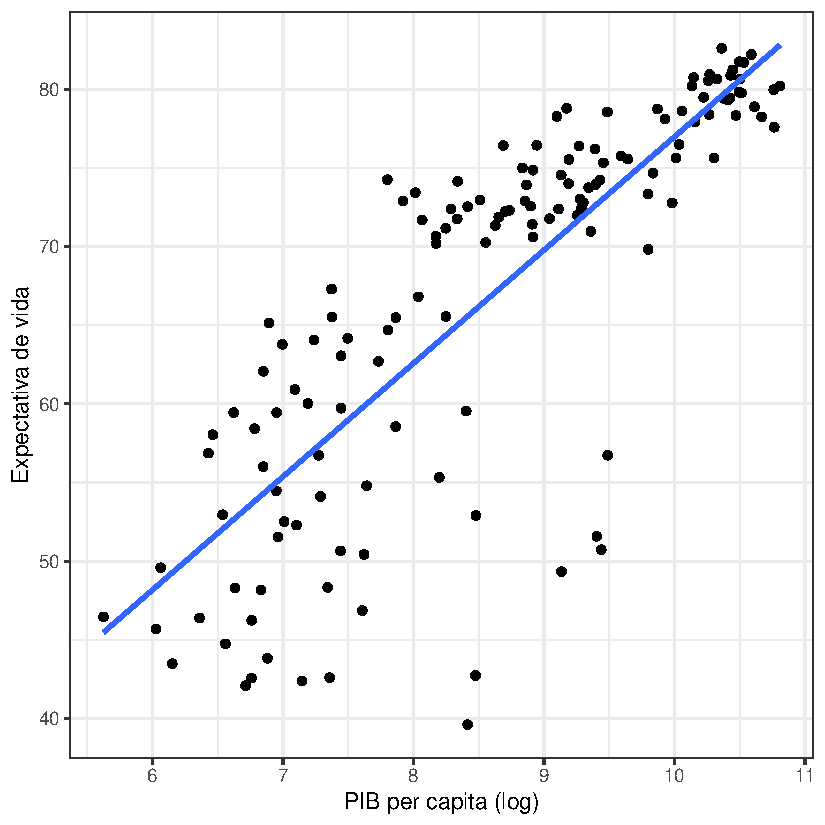
\includegraphics{arquivo_pdf_files/figure-latex/scatter2-1} \end{center}

\hypertarget{argumento-col}{%
\section{Argumento col}\label{argumento-col}}

\begin{Shaded}
\begin{Highlighting}[]
\KeywordTok{ggplot}\NormalTok{(base,}\KeywordTok{aes}\NormalTok{(}\DataTypeTok{y=}\NormalTok{lifeExp, }\DataTypeTok{x=}\KeywordTok{log}\NormalTok{(gdpPercap), }\DataTypeTok{col=}\NormalTok{continent)) }\OperatorTok{+}\StringTok{ }\KeywordTok{geom_point}\NormalTok{() }\OperatorTok{+}
\StringTok{  }\KeywordTok{geom_smooth}\NormalTok{(}\DataTypeTok{method =} \StringTok{"lm"}\NormalTok{, }\DataTypeTok{se=}\OtherTok{FALSE}\NormalTok{) }\OperatorTok{+}\StringTok{ }
\StringTok{  }\KeywordTok{labs}\NormalTok{(}\DataTypeTok{x =} \StringTok{"PIB per capita (log)"}\NormalTok{,}
       \DataTypeTok{y =} \StringTok{"Expectativa de vida"}\NormalTok{) }\OperatorTok{+}\StringTok{ }\KeywordTok{theme_bw}\NormalTok{()}
\end{Highlighting}
\end{Shaded}

\begin{center}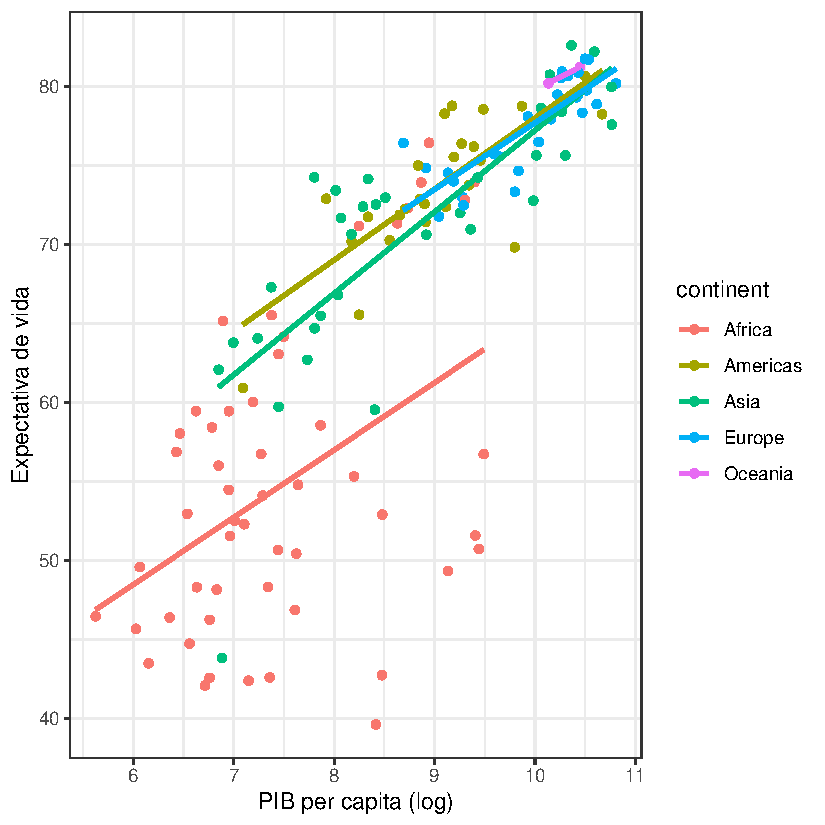
\includegraphics{arquivo_pdf_files/figure-latex/scatter3-1} \end{center}

\hypertarget{argumento-size}{%
\section{Argumento size}\label{argumento-size}}

\begin{Shaded}
\begin{Highlighting}[]
\KeywordTok{ggplot}\NormalTok{(base,}\KeywordTok{aes}\NormalTok{(}\DataTypeTok{y=}\NormalTok{lifeExp, }\DataTypeTok{x=}\KeywordTok{log}\NormalTok{(gdpPercap), }\DataTypeTok{col=}\NormalTok{continent,}\DataTypeTok{size =}\NormalTok{ pop)) }\OperatorTok{+}\StringTok{ }\KeywordTok{geom_point}\NormalTok{() }\OperatorTok{+}
\StringTok{  }\KeywordTok{geom_smooth}\NormalTok{(}\DataTypeTok{method =} \StringTok{"lm"}\NormalTok{, }\DataTypeTok{se=}\OtherTok{FALSE}\NormalTok{) }\OperatorTok{+}\StringTok{ }
\StringTok{  }\KeywordTok{labs}\NormalTok{(}\DataTypeTok{x =} \StringTok{"PIB per capta (log)"}\NormalTok{,}
       \DataTypeTok{y =} \StringTok{"Expectativa de vida"}\NormalTok{) }\OperatorTok{+}\StringTok{ }\KeywordTok{theme_bw}\NormalTok{()}
\end{Highlighting}
\end{Shaded}

\begin{center}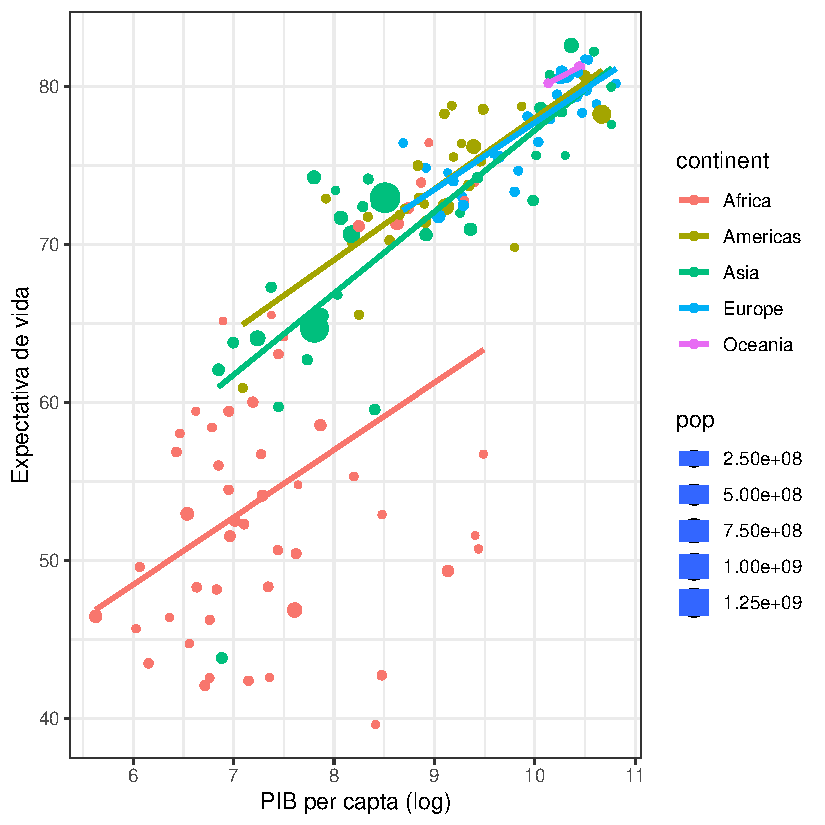
\includegraphics{arquivo_pdf_files/figure-latex/scatter4-1} \end{center}

\hypertarget{facet}{%
\section{Facet}\label{facet}}

\begin{Shaded}
\begin{Highlighting}[]
\KeywordTok{ggplot}\NormalTok{(base,}\KeywordTok{aes}\NormalTok{(}\DataTypeTok{x=}\KeywordTok{log}\NormalTok{(gdpPercap), }\DataTypeTok{y=}\NormalTok{lifeExp, }\DataTypeTok{col=}\NormalTok{continent,}
                \DataTypeTok{size =}\NormalTok{ pop)) }\OperatorTok{+}\StringTok{ }\KeywordTok{geom_point}\NormalTok{() }\OperatorTok{+}\StringTok{ }\KeywordTok{geom_smooth}\NormalTok{(}\DataTypeTok{method =} \StringTok{"lm"}\NormalTok{, }\DataTypeTok{se=}\OtherTok{FALSE}\NormalTok{) }\OperatorTok{+}\StringTok{ }
\StringTok{  }\KeywordTok{labs}\NormalTok{(}\DataTypeTok{x =} \StringTok{"PIB per capita (log)"}\NormalTok{, }\DataTypeTok{y =} \StringTok{"Expectativa de vida"}\NormalTok{) }\OperatorTok{+}\StringTok{ }\KeywordTok{theme_bw}\NormalTok{() }\OperatorTok{+}\StringTok{ }
\StringTok{  }\KeywordTok{facet_grid}\NormalTok{(}\OperatorTok{~}\NormalTok{continent)}
\end{Highlighting}
\end{Shaded}

\begin{center}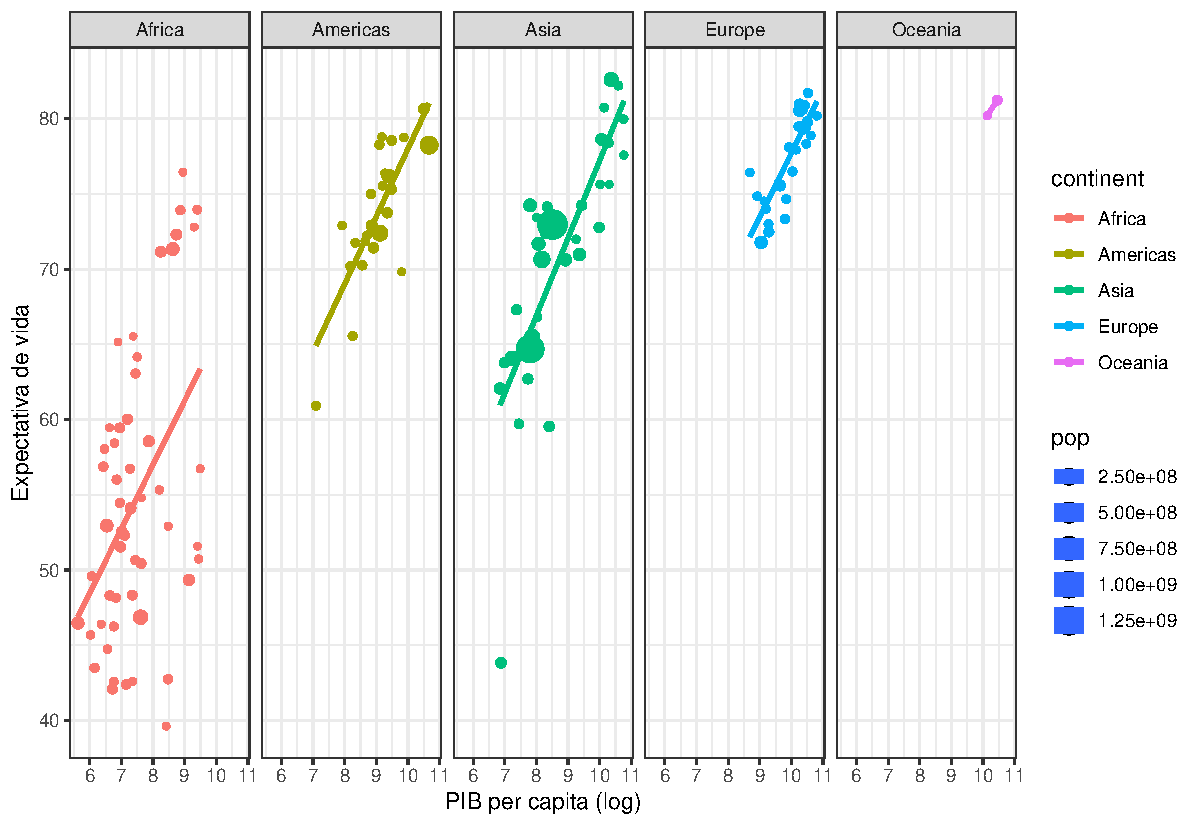
\includegraphics{arquivo_pdf_files/figure-latex/scatter5-1} \end{center}

\hypertarget{tabela-interativa-buxf4nus}{%
\section{Tabela interativa (Bônus!)}\label{tabela-interativa-buxf4nus}}

Conhecimentos extras. Clique \href{https://rstudio.github.io/DT/}{aqui}
para conhecer mais do pacote DT.

\begin{Shaded}
\begin{Highlighting}[]
\NormalTok{DT}\OperatorTok{::}\KeywordTok{datatable}\NormalTok{(base, }\DataTypeTok{options =} \KeywordTok{list}\NormalTok{(}\DataTypeTok{pageLength =} \DecValTok{5}\NormalTok{), }\DataTypeTok{class =} \StringTok{'cell-border stripe'}\NormalTok{)}
\end{Highlighting}
\end{Shaded}

\includegraphics{arquivo_pdf_files/figure-latex/datatable-1.pdf}

\hypertarget{tarefa-de-casa}{%
\section{Tarefa de casa}\label{tarefa-de-casa}}

\begin{enumerate}
\def\labelenumi{\arabic{enumi})}
\item
  Crie um boxplot para a variável expectativa de vida
\item
  Crie um boxplot para a variável expectativa de vida e cada continentes
  em um mesmo painel
\item
  Faça o mesmo que a questão 2, mas dessa vez use facet
\item
  Insira título nos gráficos, mude o nome dos eixos e coloque outro tema
\item
  Faça um gráfico de linha com a evolução do PIB per capta do Brasil,
  Argentina, Portugal e China
\end{enumerate}

\hypertarget{criando-gruxe1ficos-com-esquisse}{%
\section{Criando gráficos com
Esquisse}\label{criando-gruxe1ficos-com-esquisse}}

esquisser(viewer = ``browser'')

\begin{figure}

{\centering 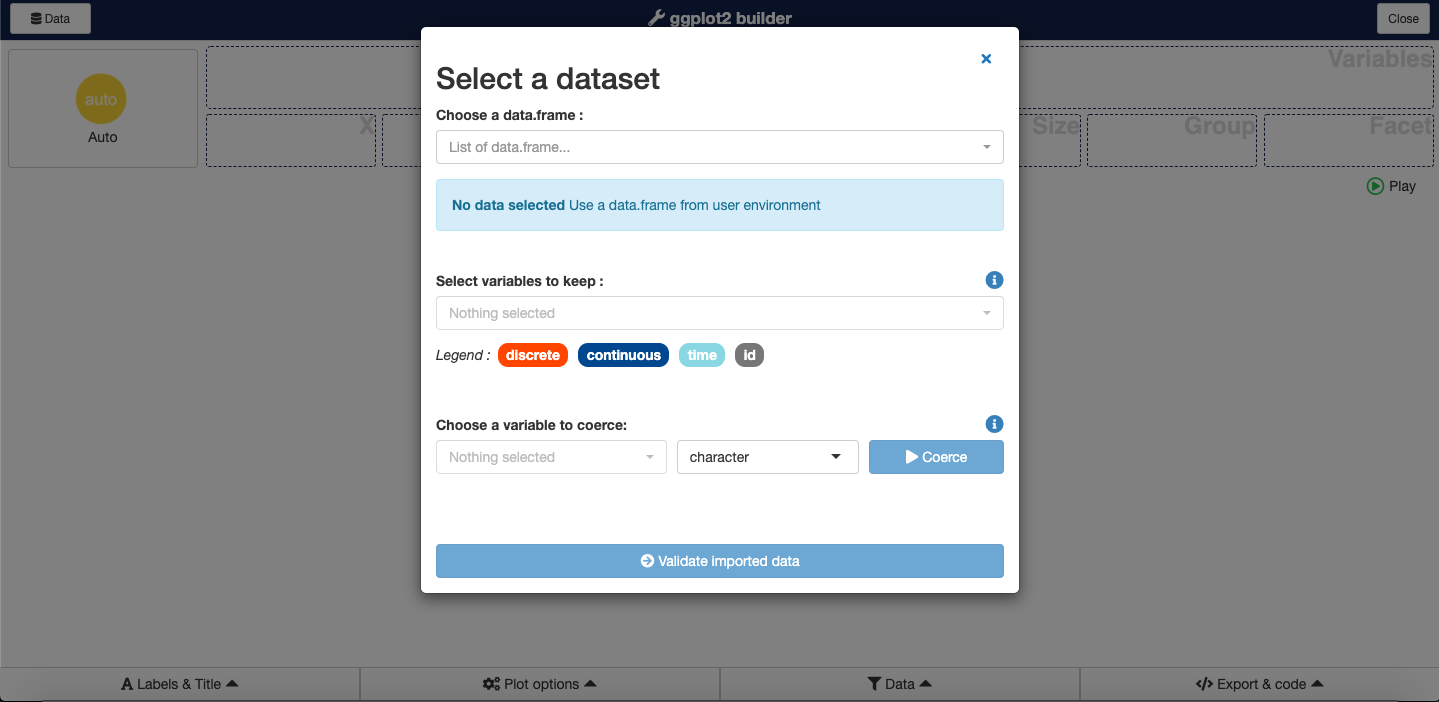
\includegraphics[width=0.9\linewidth,height=0.7\textheight]{imagem/esquisse} 

}

\caption{ }\label{fig:imagem_esquisse, figures-side}
\end{figure}

\hypertarget{gerando-gruxe1ficos-interativos}{%
\section{Gerando gráficos
interativos}\label{gerando-gruxe1ficos-interativos}}

Vamos resgatar um gráfico que fizemos lá atrás

\begin{Shaded}
\begin{Highlighting}[]
\KeywordTok{library}\NormalTok{(plotly)}

\NormalTok{grafico <-}\StringTok{ }\KeywordTok{ggplot}\NormalTok{(base,}\KeywordTok{aes}\NormalTok{(}\DataTypeTok{y=}\NormalTok{lifeExp, }\DataTypeTok{x=}\KeywordTok{log}\NormalTok{(gdpPercap), }\DataTypeTok{col=}\NormalTok{continent)) }\OperatorTok{+}\StringTok{ }\KeywordTok{geom_point}\NormalTok{() }\OperatorTok{+}
\StringTok{  }\KeywordTok{labs}\NormalTok{(}\DataTypeTok{x =} \StringTok{"PIB per capita (log)"}\NormalTok{,}
       \DataTypeTok{y =} \StringTok{"Expectativa de vida"}\NormalTok{) }\OperatorTok{+}\StringTok{ }\KeywordTok{theme_bw}\NormalTok{()}

\KeywordTok{ggplotly}\NormalTok{(grafico)}
\end{Highlighting}
\end{Shaded}

\begin{center}\includegraphics{arquivo_pdf_files/figure-latex/plotly2-1} \end{center}

\hypertarget{para-aprender-mais}{%
\section{Para aprender mais}\label{para-aprender-mais}}

\begin{itemize}
\tightlist
\item
  \href{https://rstudio.com/wp-content/uploads/2015/03/ggplot2-cheatsheet.pdf}{GGPlot2
  cheat sheet}
\item
  \href{https://www.youtube.com/watch?v=IPyjHKe30eo}{GGPlot2 - LAPEI}
\item
  \href{https://plotly.com/}{Plotly}
\item
  \href{https://www.datanovia.com/en/blog/gganimate-how-to-create-plots-with-beautiful-animation-in-r/}{Blog
  Datanovia}
\item
  \href{https://rkabacoff.github.io/datavis/Interactive.html}{Datavis
  with R} Apresentação feita com Rmarkdown, usando pacote xaringã
\end{itemize}

\hypertarget{obrigado}{%
\section{Obrigado}\label{obrigado}}

\textbf{Daniel Pagotto} \textbar{}
\href{mailto:danielppagotto@gmail.com}{\nolinkurl{danielppagotto@gmail.com}}
\textbar{}
\href{https://www.linkedin.com/in/daniel-do-prado-pagotto-bab62a50/}{LinkedIn}

\end{document}
